\chapter{HASIL DAN PEMBAHASAN}
\section{Hasil}
\noindent

Tahapan ini merupakan tahapan yang berisi tentang penjelasan bagaimana game ini dapat bekerja sesuai dengan yang diharapkan dan dapat berjalan dengan baik. Tahapan ini meliputi perancangan perangkat lunak, bagian program yang penting dan implementasi sehingga dapat dipahami dengan baik dan mengetahui cara menggunakannya.

\subsection{Desain Perangkat Lunak}

\begin{enumerate}
    \item Tampilan \textit{Connecting Network} \\
    Tampilan \textit{connecting network} adalah tampilan awal disaat game dibuka, pada tampilan ini akan menghubungkan player ke jaringan photon .
    \begin{figure}[h]
        \centering
        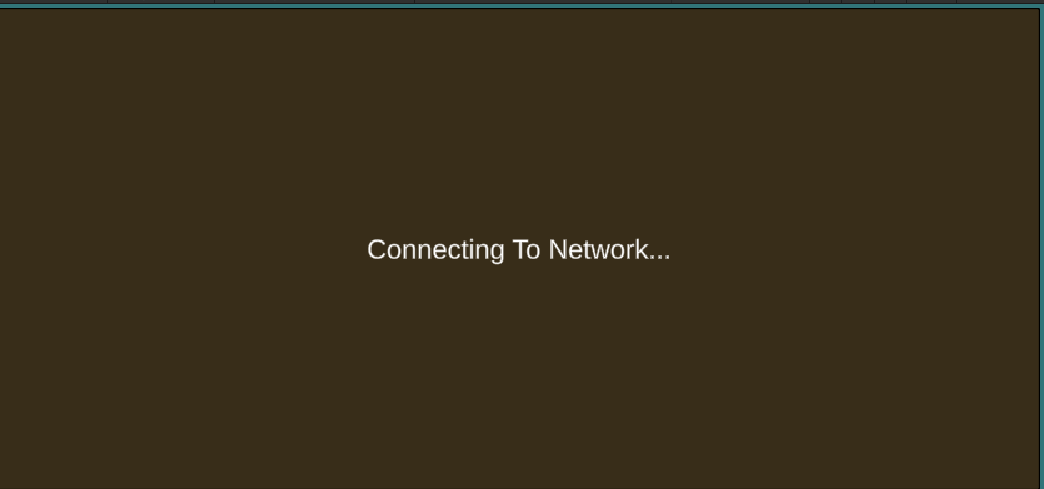
\includegraphics[width=10cm]{connecting.png}
        \caption{Tampilan \textit{Connecting Network}}
        \label{fig:connecting}
    \end{figure}
    \item Tampilan Set \textit{Nickname} \\
    Set \textit{nickname menu} merupakan letak dimana player harus mengisikan nama untuk memberikan identitas nama dari player. 
    \newpage
    \begin{figure}[h]
        \centering
        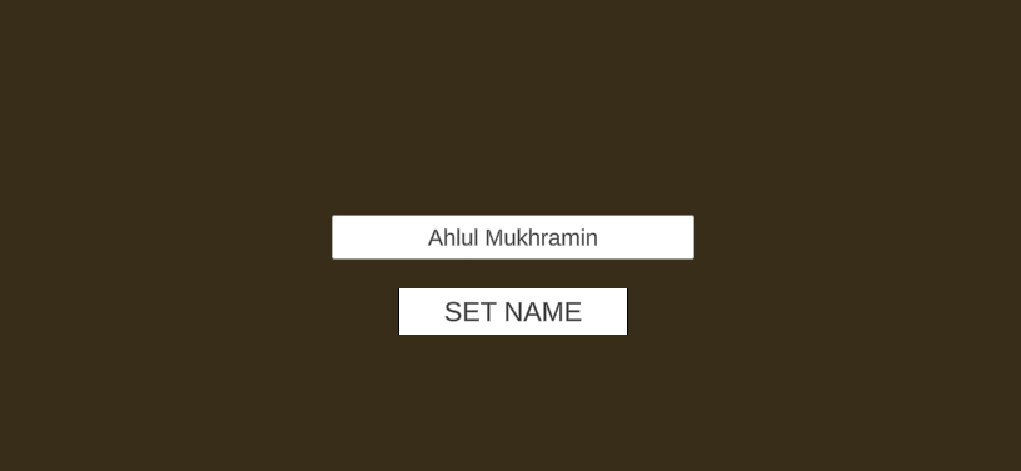
\includegraphics[width=10cm]{setnama.png}
        \caption{Tampilan Mengatur Nama}
        \label{fig:setnama}
    \end{figure}
    \item Tampilan Menu Utama\\
    Tampilan menu utama adalah tampilan menu yang terdapat button "cari room" untuk mencari room yang tersedia, "buat room" untuk membuat room sebagai master room,  "thanks to" untuk melihat \textit{credit} asset yang digunakan dan "Keluar" untuk menutup game.
    \begin{figure}[h]
        \centering
        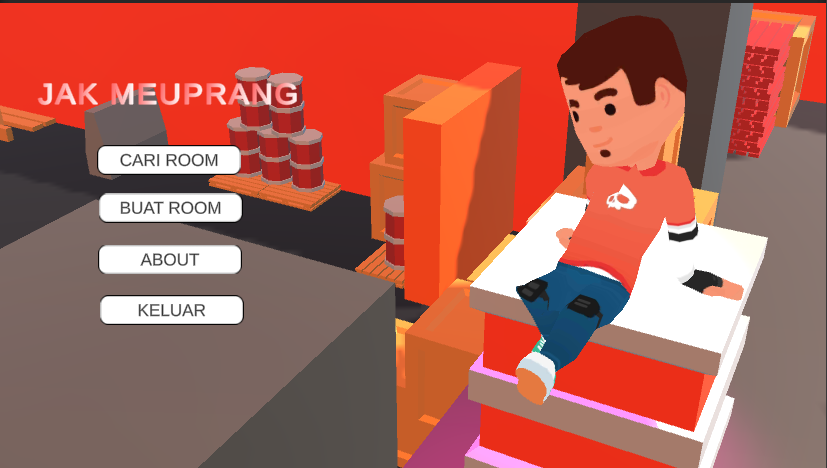
\includegraphics[width=10cm]{menuutama.png}
        \caption{Tampilan Menu Utama}
        \label{fig:menutama}
    \end{figure}
    \item Tampilan Pencarian Room\\
    Pencarian room merupakan menu untuk mencari room yang tersedia yang dibuat oleh player lain untuk memainkan game bersama.
    \newpage
    \begin{figure}[h]
        \centering
        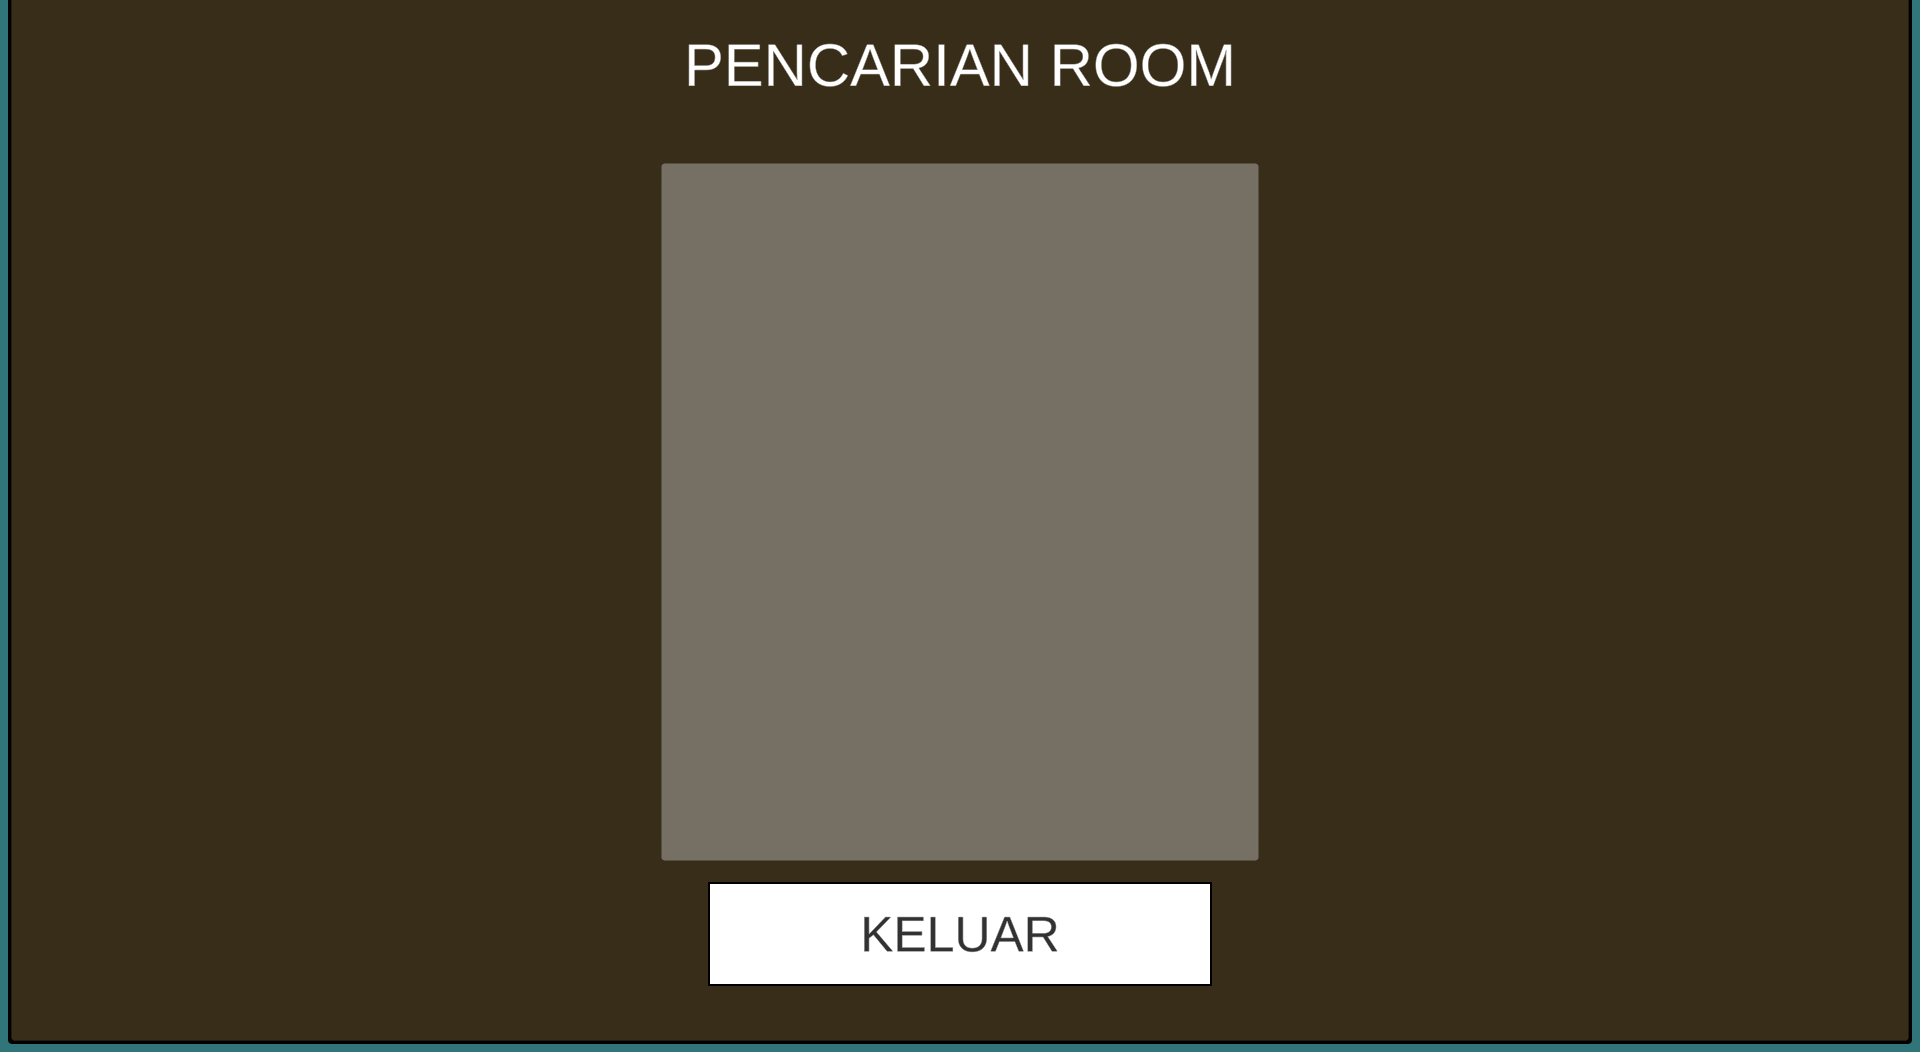
\includegraphics[width=10cm]{pencarian.png}
        \caption{Tampilan Pencarian}
        \label{fig:pencarian}
    \end{figure}
    \item Tampilan Buat Room \\
    Buat room merupakan menu untuk membuat room bagi player ingin menjadi host pada room tersebut, pada menu buat room ini player harus mengisikan nama room terlebih dahulul seperti gambar \ref{fig:namaroom}.
    \begin{figure}[h]
        \centering
        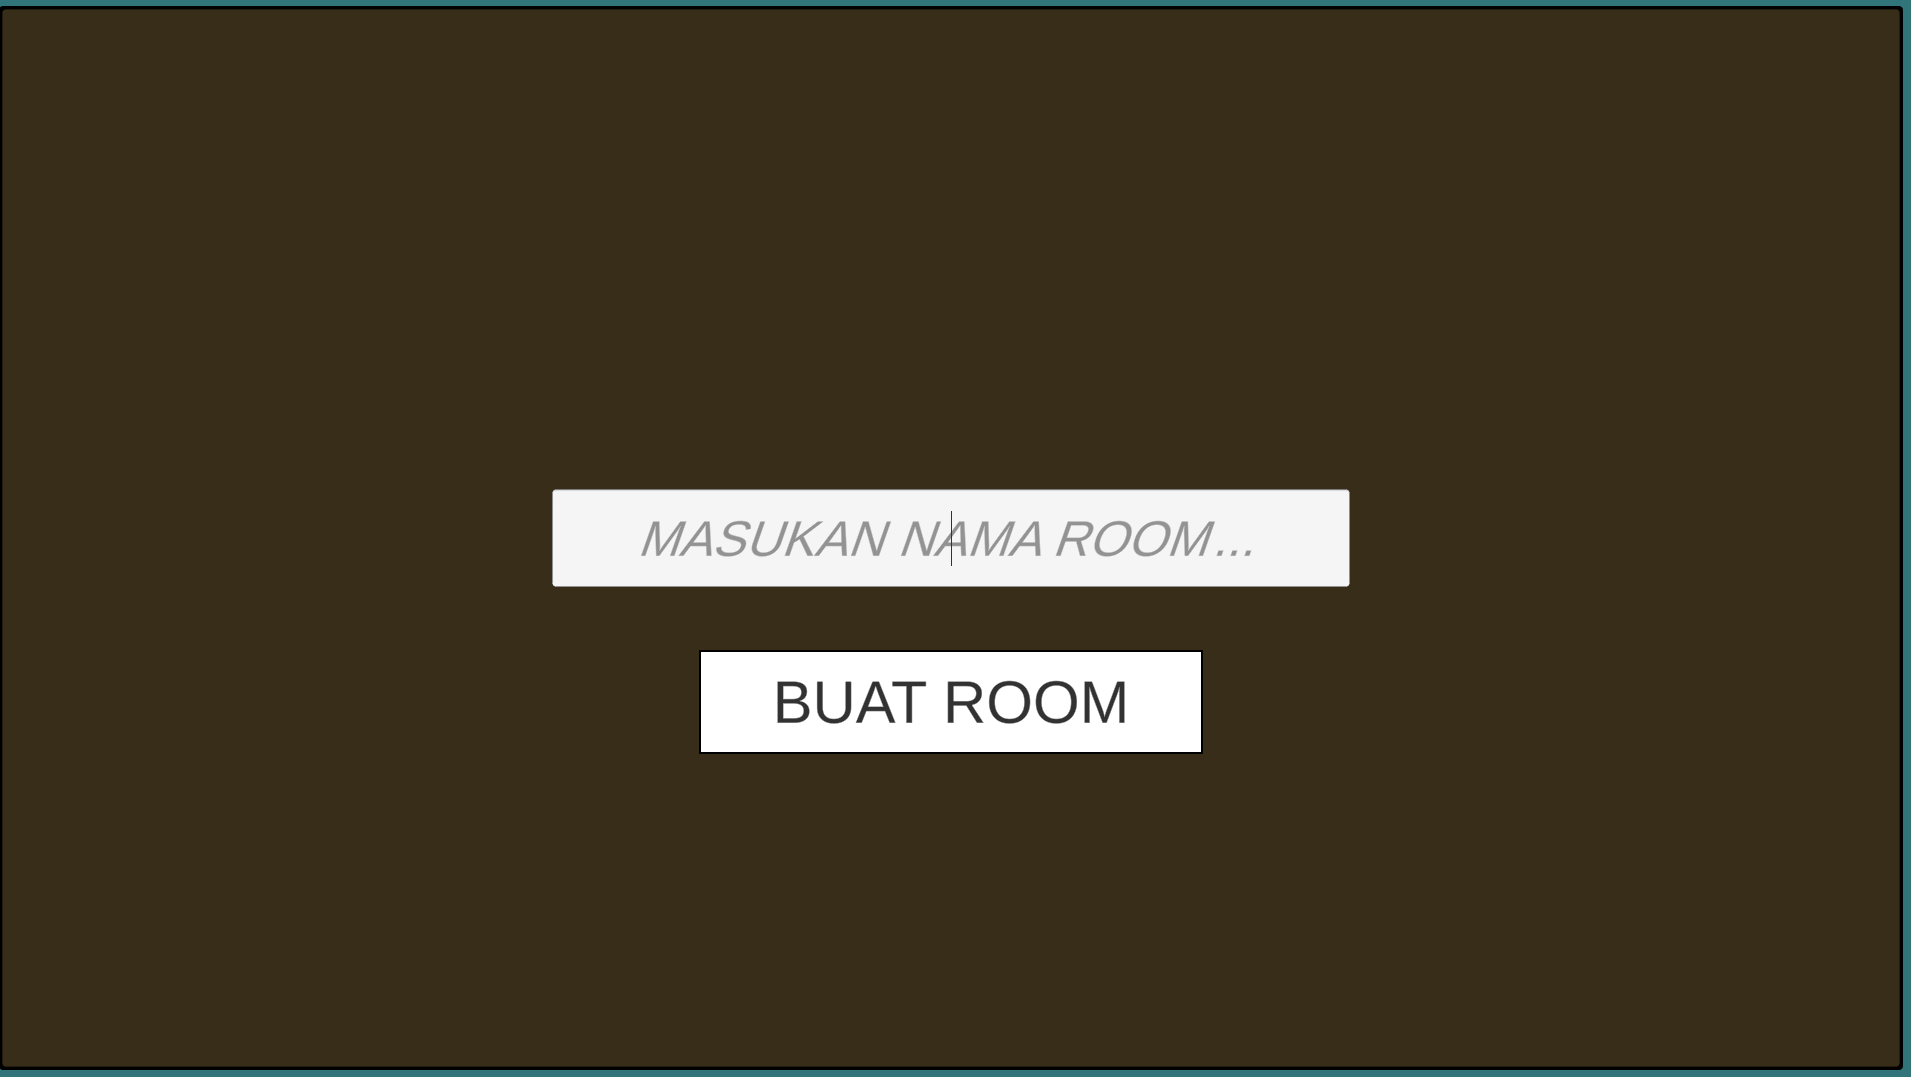
\includegraphics[width=10cm]{namaroom.png}
        \caption{Tampilan Buat Nama Room}
        \label{fig:namaroom}
    \end{figure}
    \\ setelah player telah mengisikan nama room maka akan menampilkan \textit{instance} baru yang berisi player player pada room tersebut, dan hanya host room yang dapat memulai permainannya.
    \newpage
    \begin{figure}[h]
        \centering
        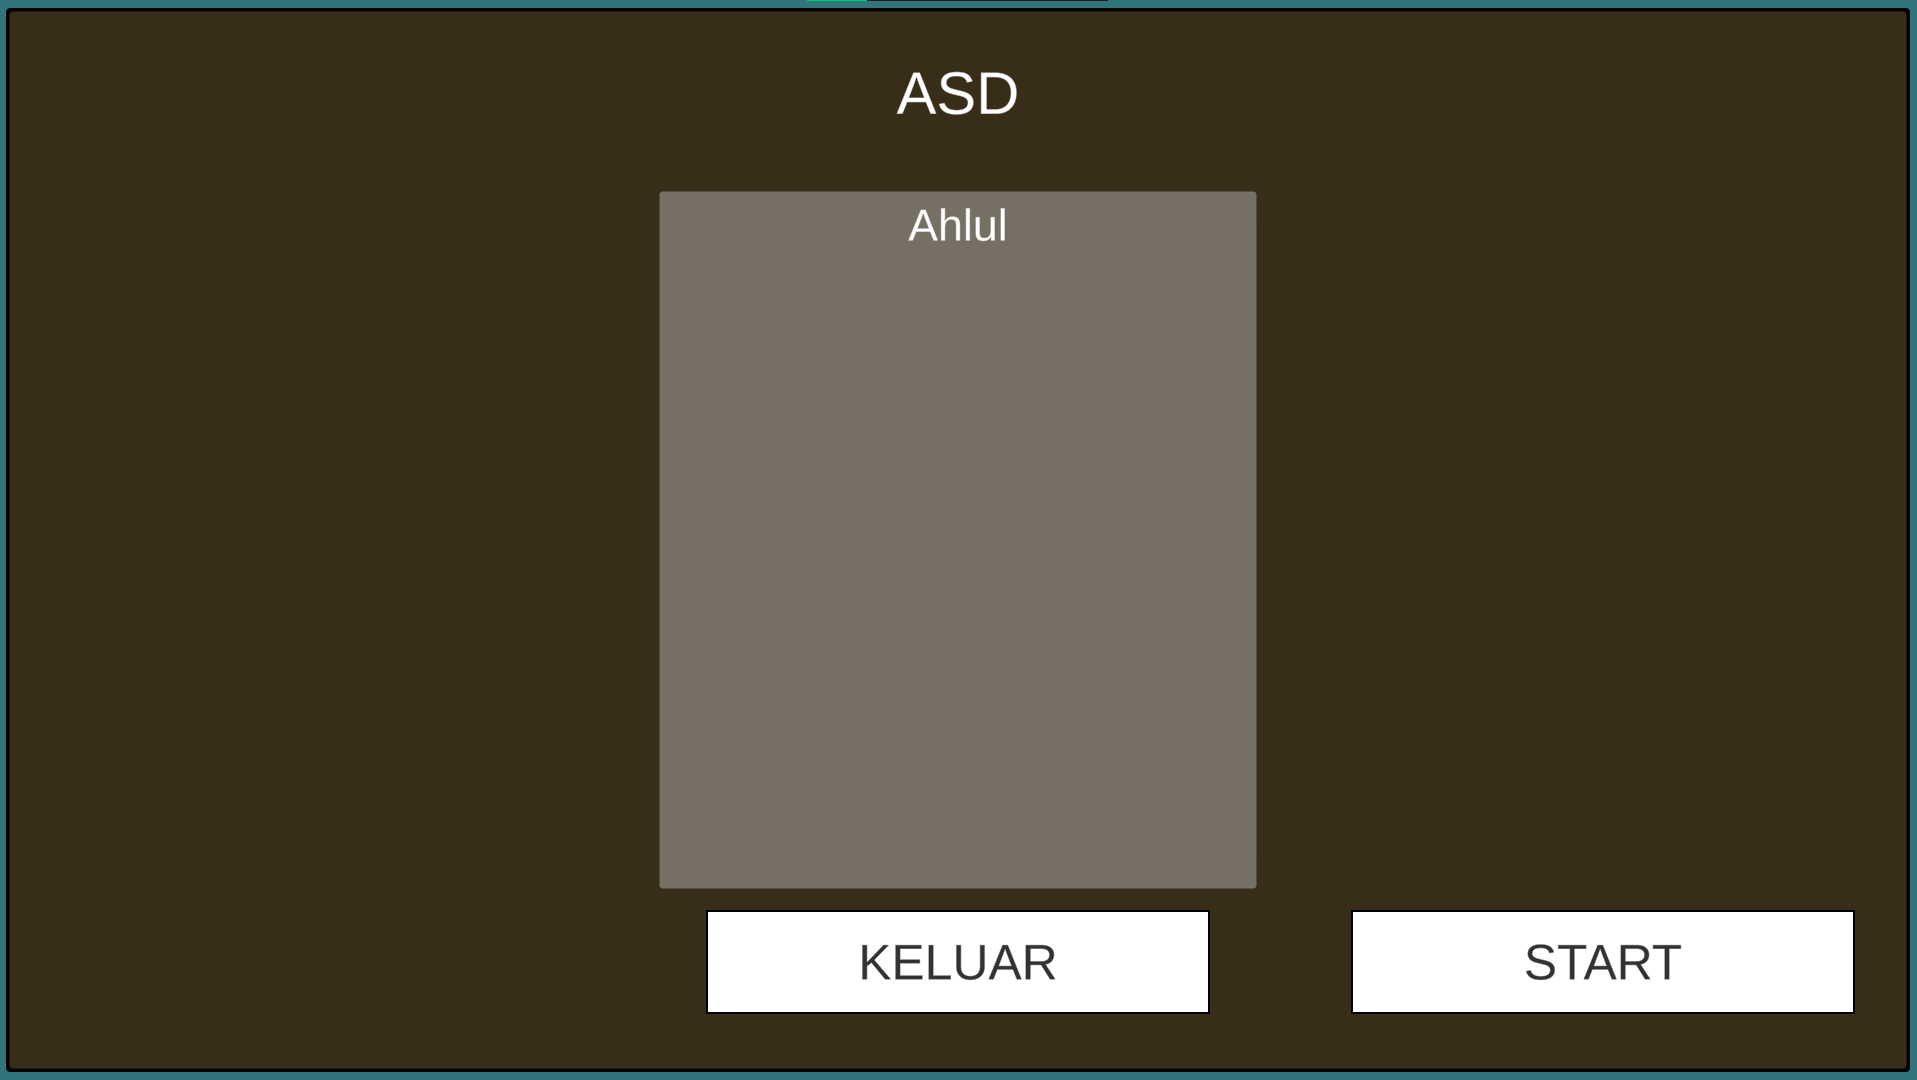
\includegraphics[width=10cm]{roomdone.png}
        \caption{Tampilan Room Telah Dibuat}
        \label{fig:roomdone}
    \end{figure}
    \item Tampilan Credit/About \\
    Tampilan ini merupakan tampilan informasi dari asset asset mana saja yang digunakan sebagai informasi.
    \begin{figure}[h]
        \centering
        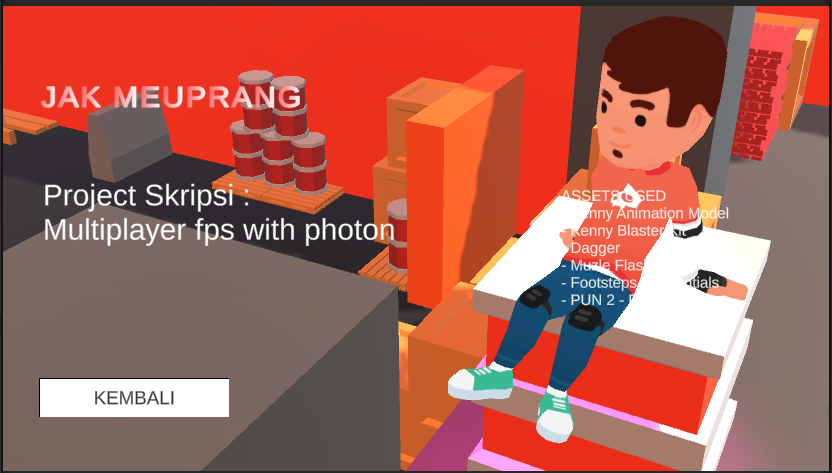
\includegraphics[width=10cm]{thanksto.png}
        \caption{Tampilan About}
        \label{fig:thanksto}
    \end{figure}
    \item Tampilan Gameplay \\
    Tampilan gameplay berisi permainan yang merupakan bagian area gameplay, pada tampilan gameplay ini menampilkan \textit{head up display} (HUD) seperti tampilan health, weapon overheat, player lain dan leaderboard.
    \newpage
    \begin{figure}[h]
        \centering
        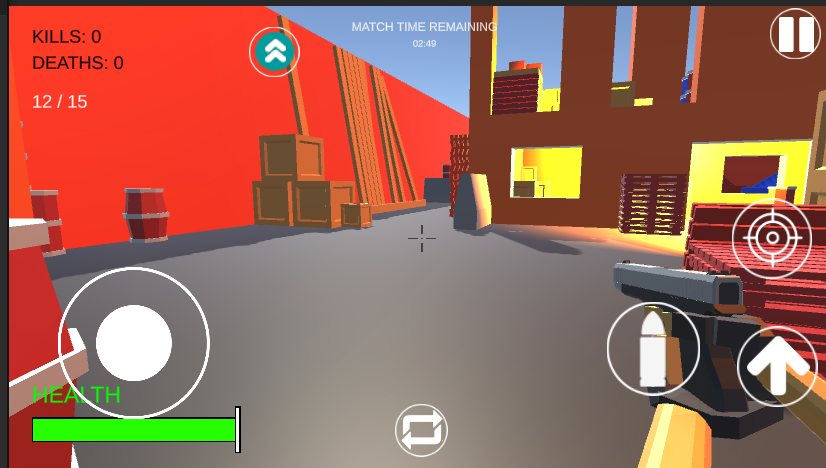
\includegraphics[width=10cm]{gameplay.png}
        \caption{Tampilan Gameplay}
        \label{fig:gameplay}
    \end{figure}
    \item Tampilan Round Over \\
    Tampilan ini ditampilkan jika waktu yang sudah ditentukan habis maka permainan telah berakhir dan player harus keluar untuk membuat room baru.
    \begin{figure}[h]
        \centering
        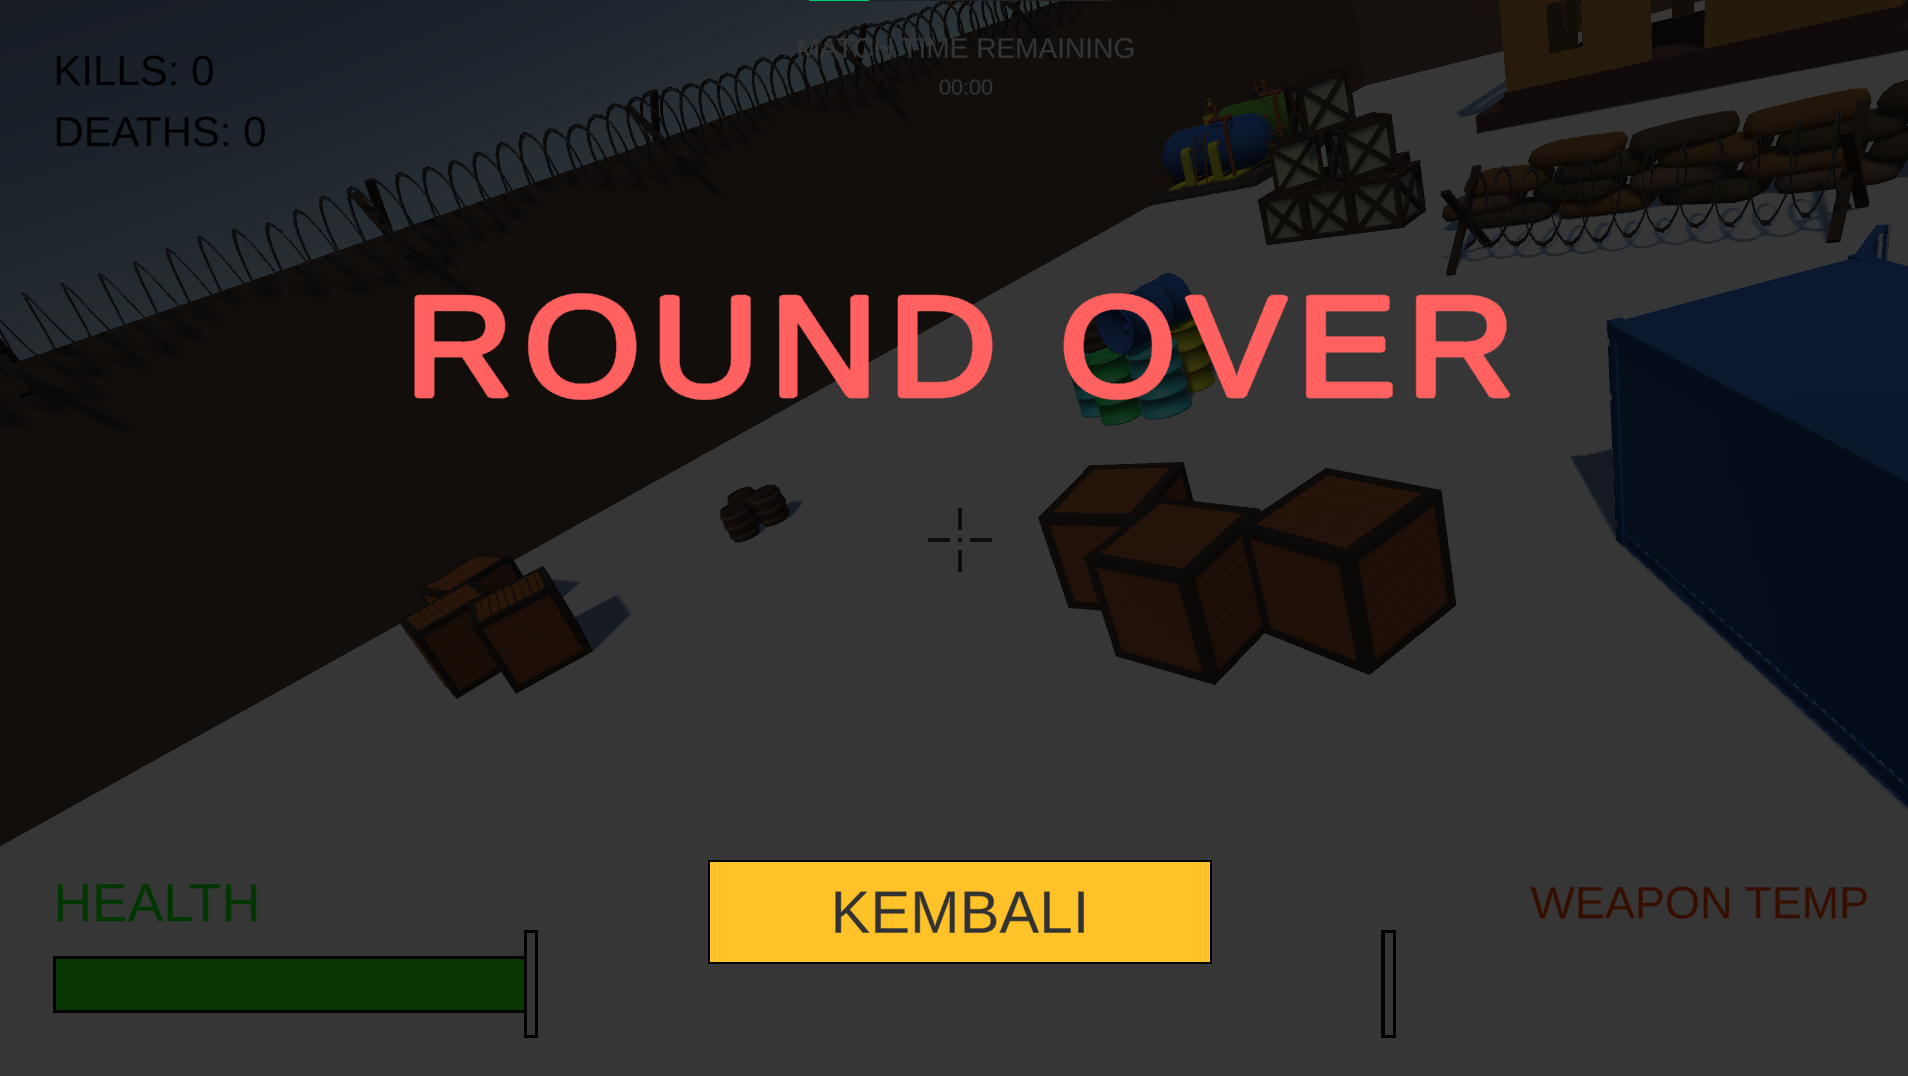
\includegraphics[width=10cm]{roundover.png}
        \caption{Tampilan Round Over}
        \label{fig:roundover}
    \end{figure}
\end{enumerate}

\subsection{\textit{Asset}}
\noindent

Sebuah permainan tidak luput dari berbagai asset karena asset ini adalah bahan bahan yang digunakan pada dalam pembuatan game ini untuk memperbagus tampilan dari game itu sendiri. Asset yang digunakan disini adalah asset gratis dari beberapa platform yang disediakan gratis. Berikut adalah beberapa asset utama yang digunakan dalam pembuatan game "JakMeuprang".
\newpage
\begin{enumerate}
    \item Karakter \\
    Adapun karakter yang digunakan dalam pembuatan game ini memiliki dua karakter yang memiliki animasi yang sama.
    \begin{table}[h!]
        \centering
        \caption{Karakter}\label{tbl:karakter}
        \begin{tabular}{ | c | c | m{6cm} | m{6cm} | }
            \hline
            No & Karakter & Nama \\ \hline
            1 &
            \begin{minipage}{.2\textwidth}
                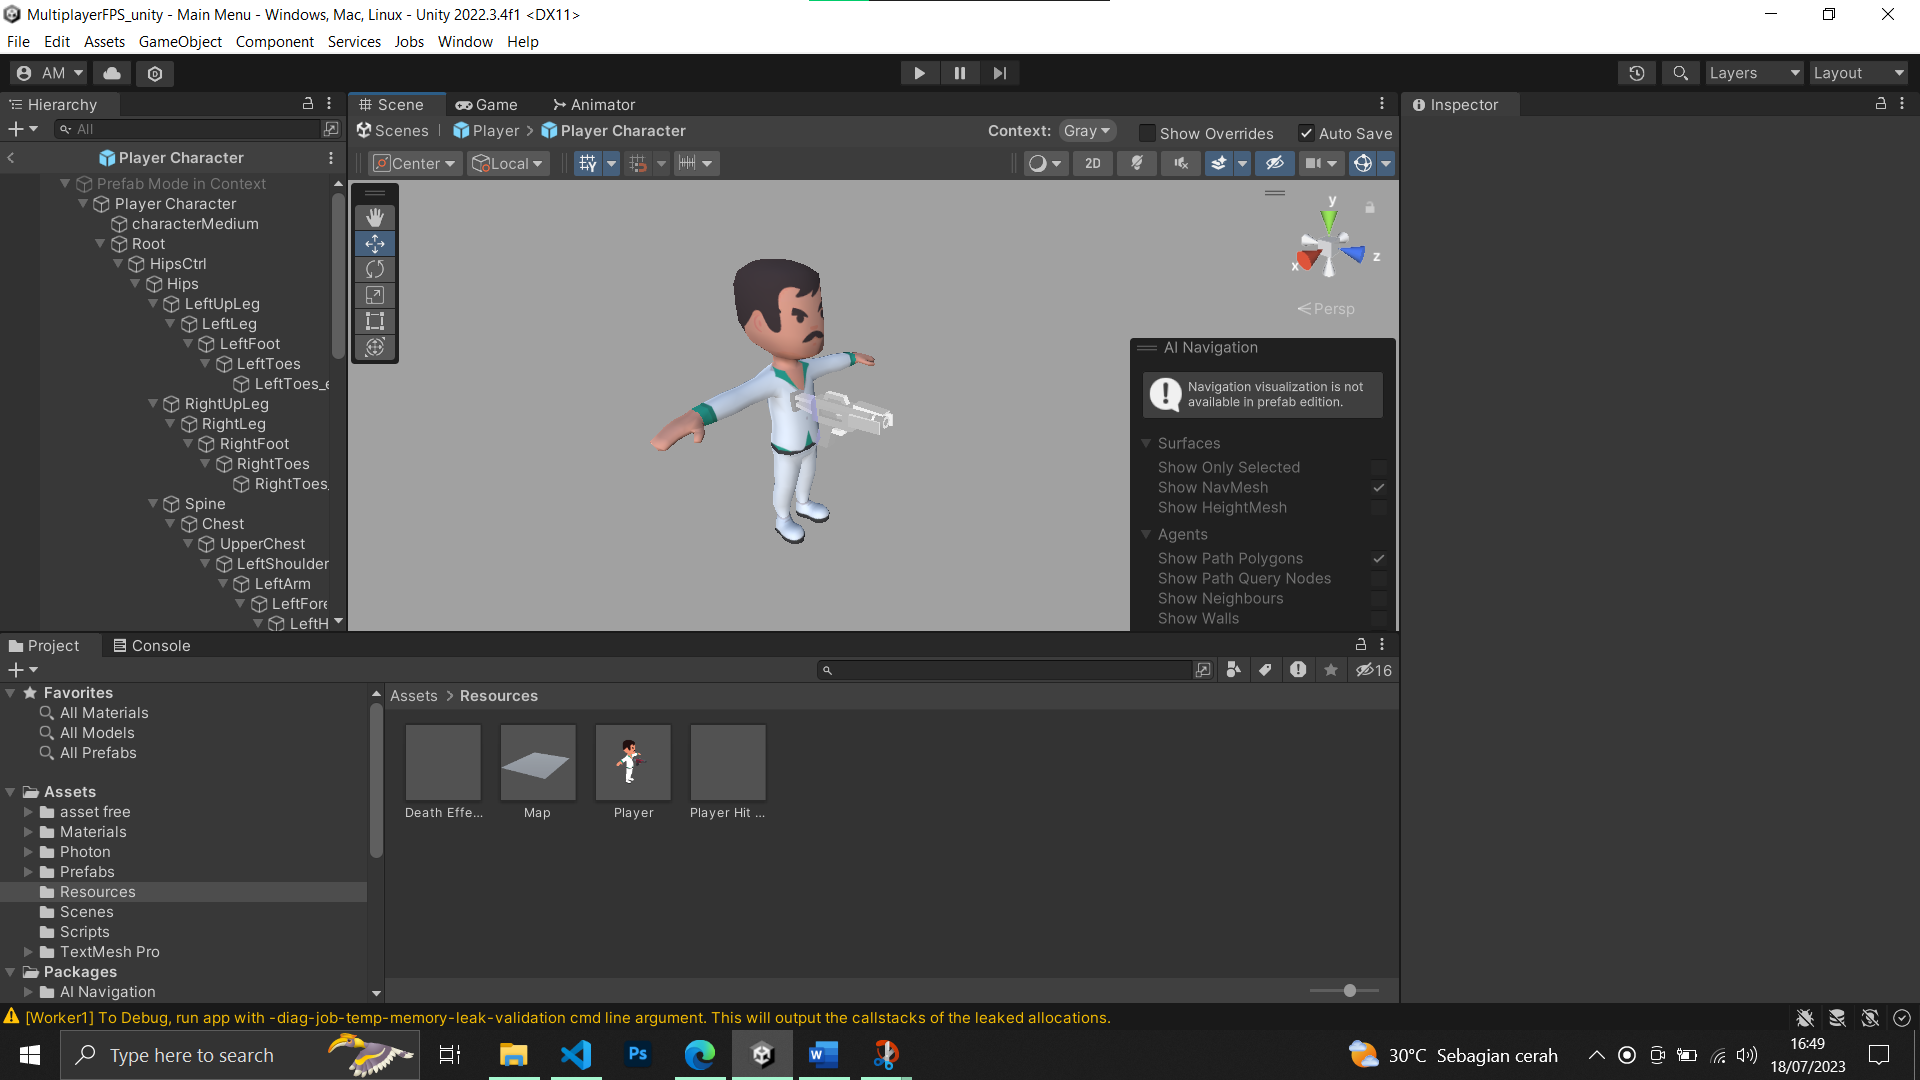
\includegraphics[width=\linewidth, height=60mm, ]{karakter1.png}
            \end{minipage}
            &
            \begin{minipage}{6cm}
                Criminal Karakter
            \end{minipage}
            \\ \hline
            2 &
        \begin{minipage}{.2\textwidth}
            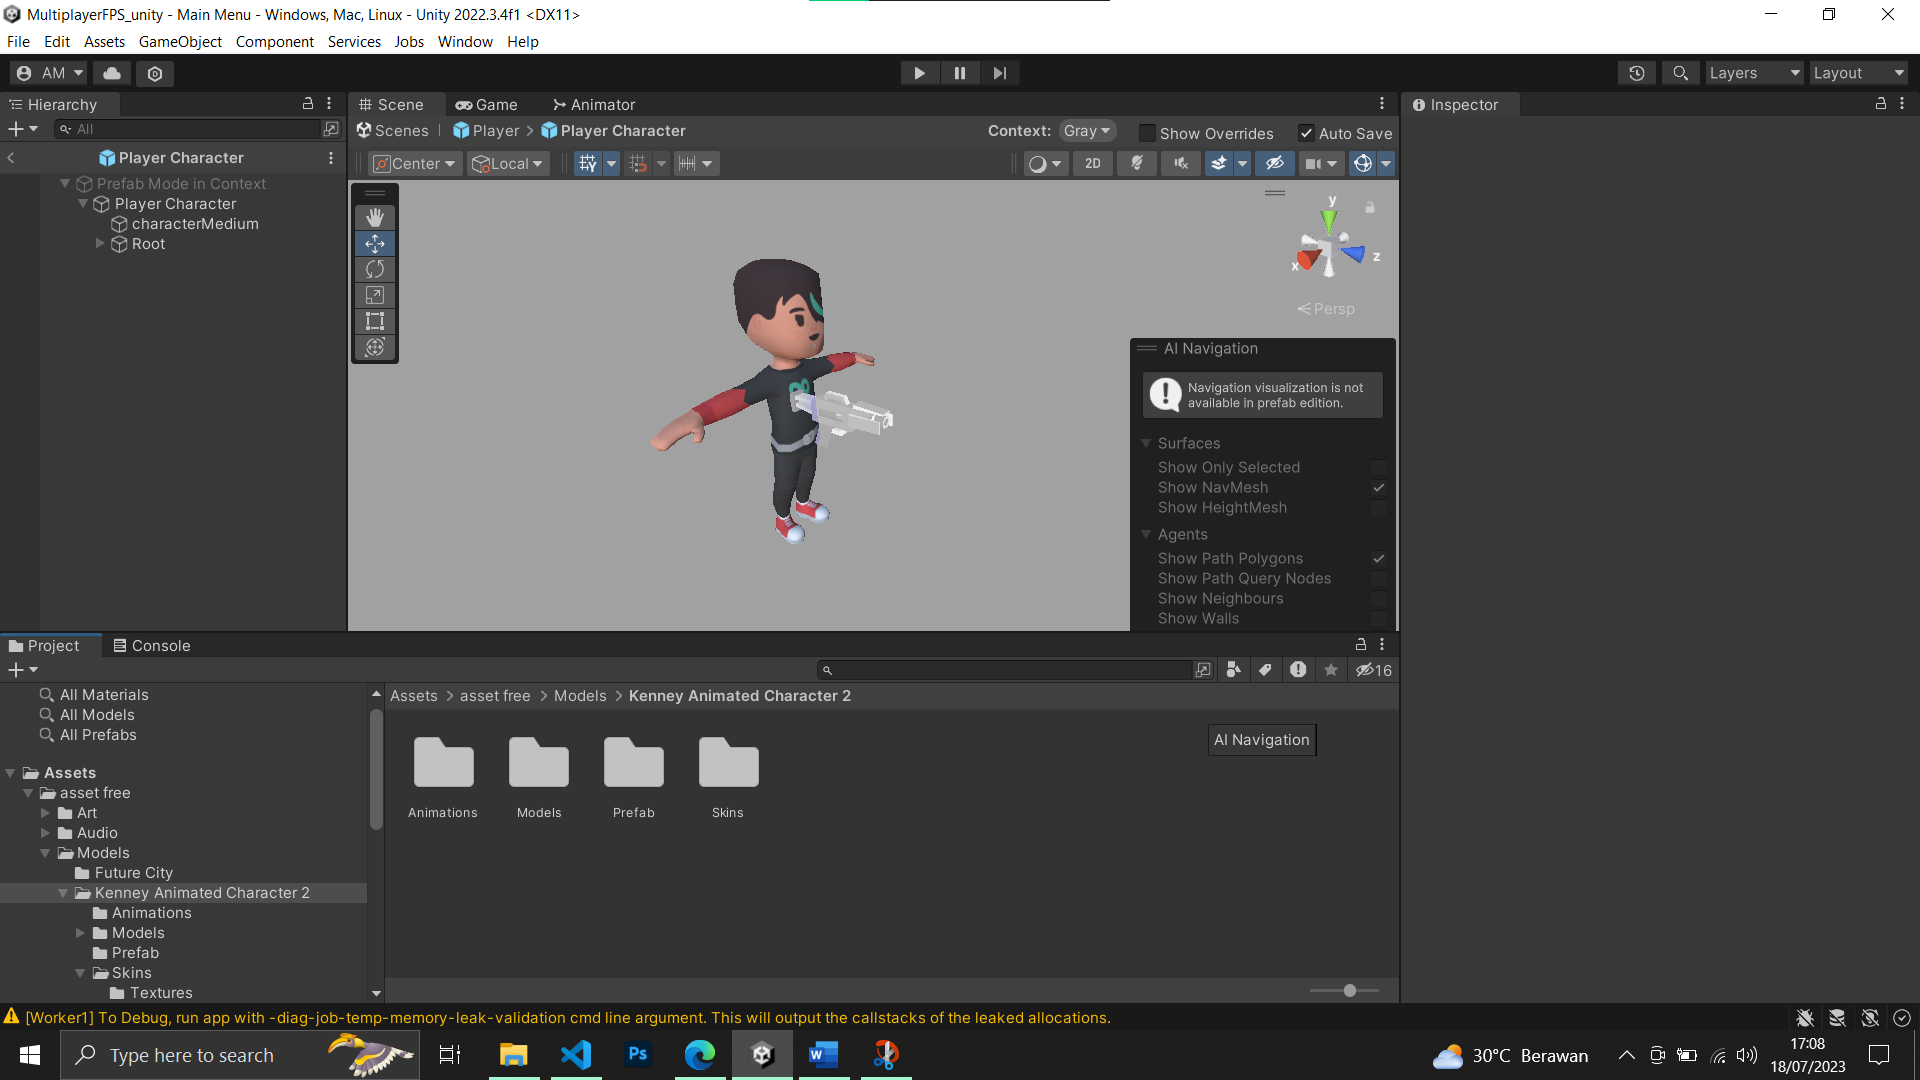
\includegraphics[width=\linewidth, height=60mm]{karakter2.png}
        \end{minipage}
        &
        \begin{minipage}{6cm}
            Skater Karakter
        \end{minipage}
        \\ \hline
        \end{tabular}
    \end{table}
    \newpage
    \item Weapon \\
    \begin{table}[h!]
        \centering
        \caption{Weapon}\label{tbl:weapon}
        \begin{tabular}{ | c | c | m{6cm} | m{6cm} | }
            \hline
            No & Weapon & Nama \\ \hline
            1 &
            \begin{minipage}{.2\textwidth}
                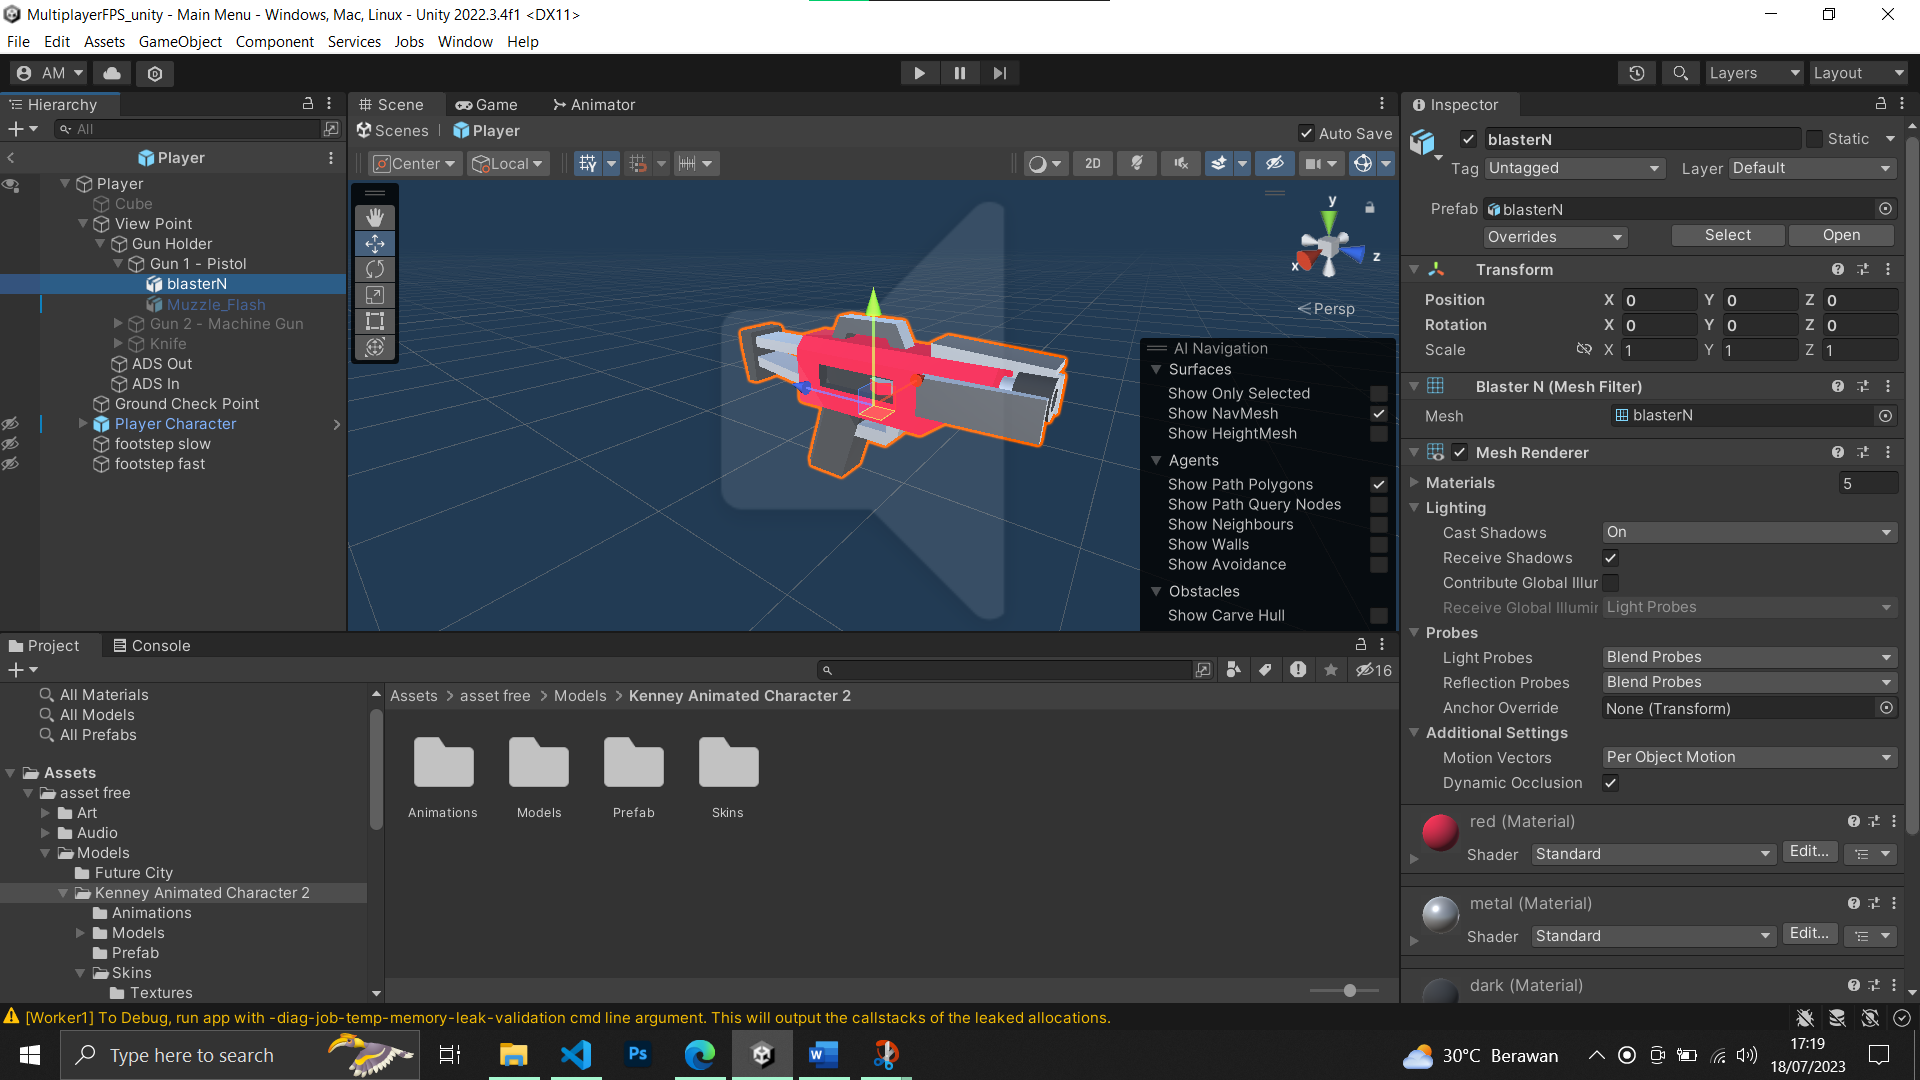
\includegraphics[width=\linewidth, height=60mm, ]{weapon1.png}
            \end{minipage}
            &
            \begin{minipage}{6cm}
                Pistol
            \end{minipage}
            \\ \hline
            2 &
        \begin{minipage}{.2\textwidth}
            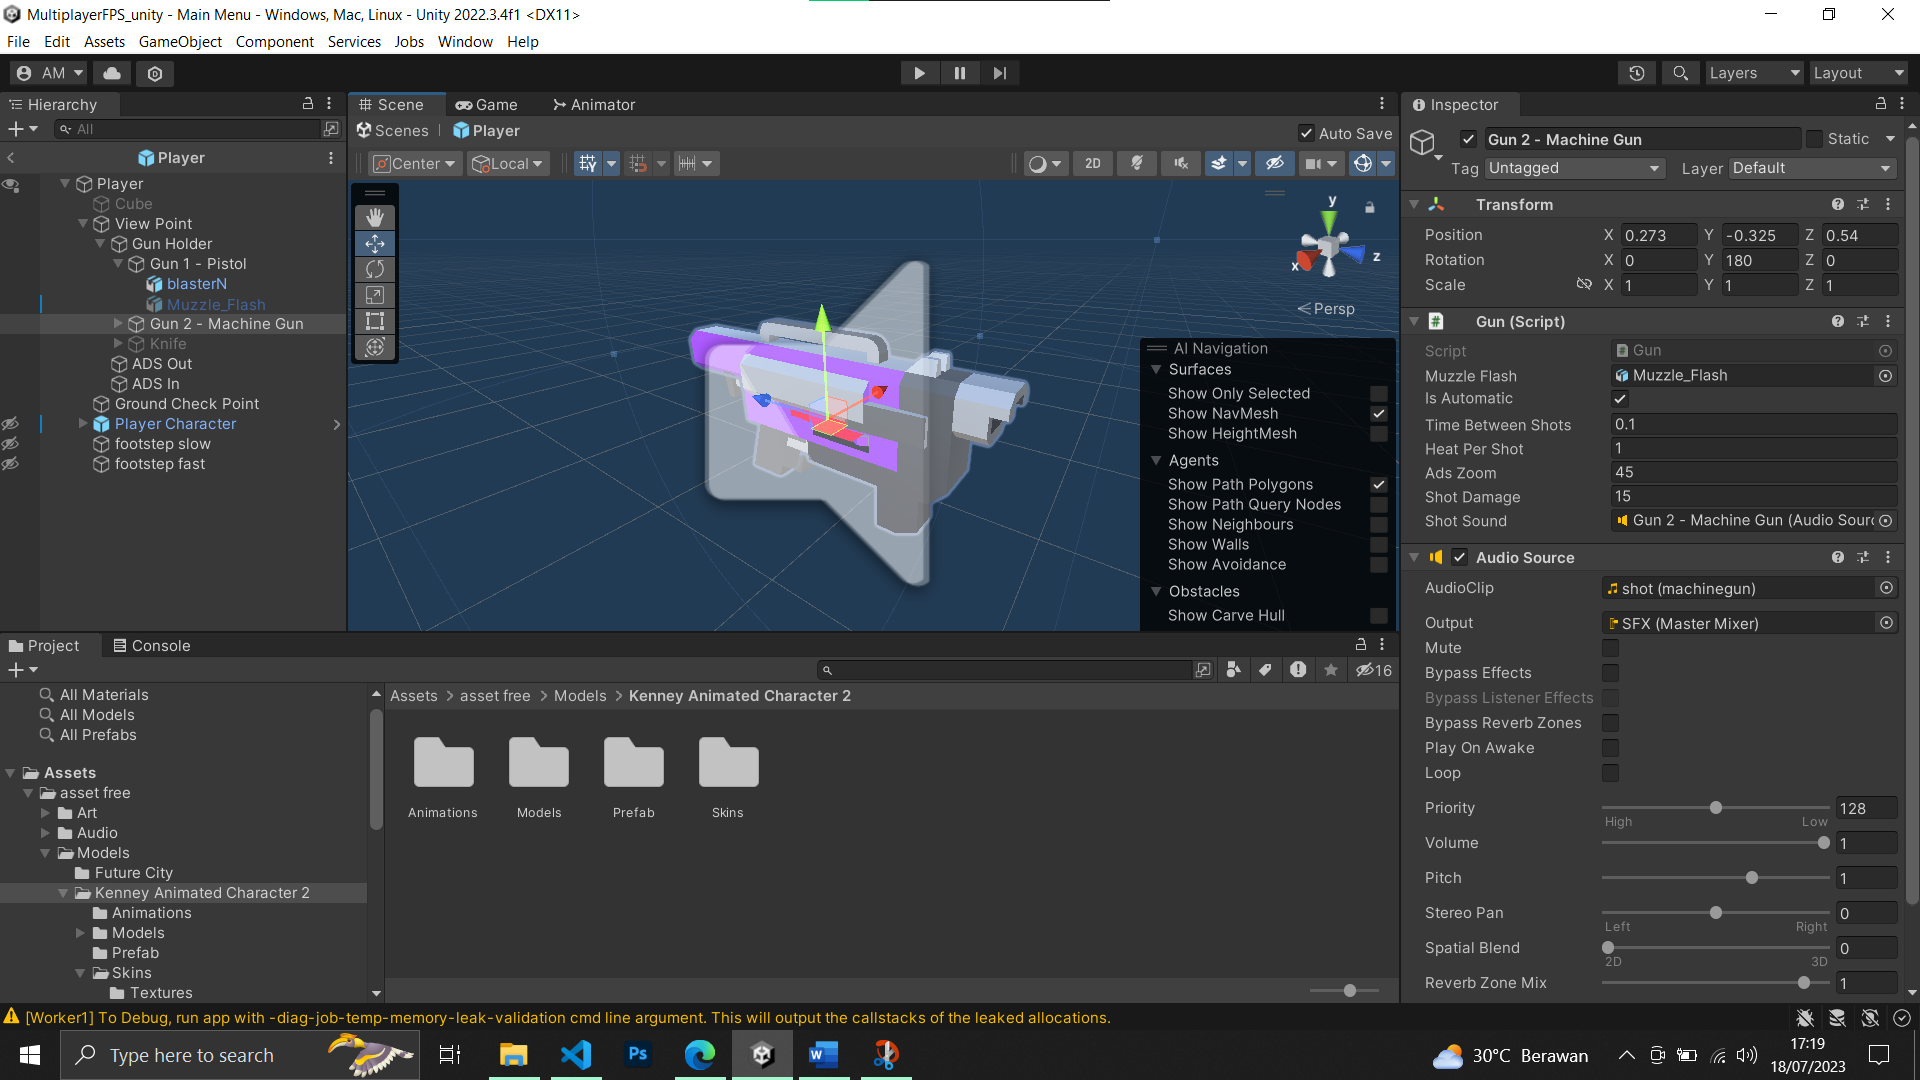
\includegraphics[width=\linewidth, height=60mm]{weapon2.png}
        \end{minipage}
        &
        \begin{minipage}{6cm}
            Smg Rifle
        \end{minipage}
        \\ \hline
        3 &
        \begin{minipage}{.2\textwidth}
            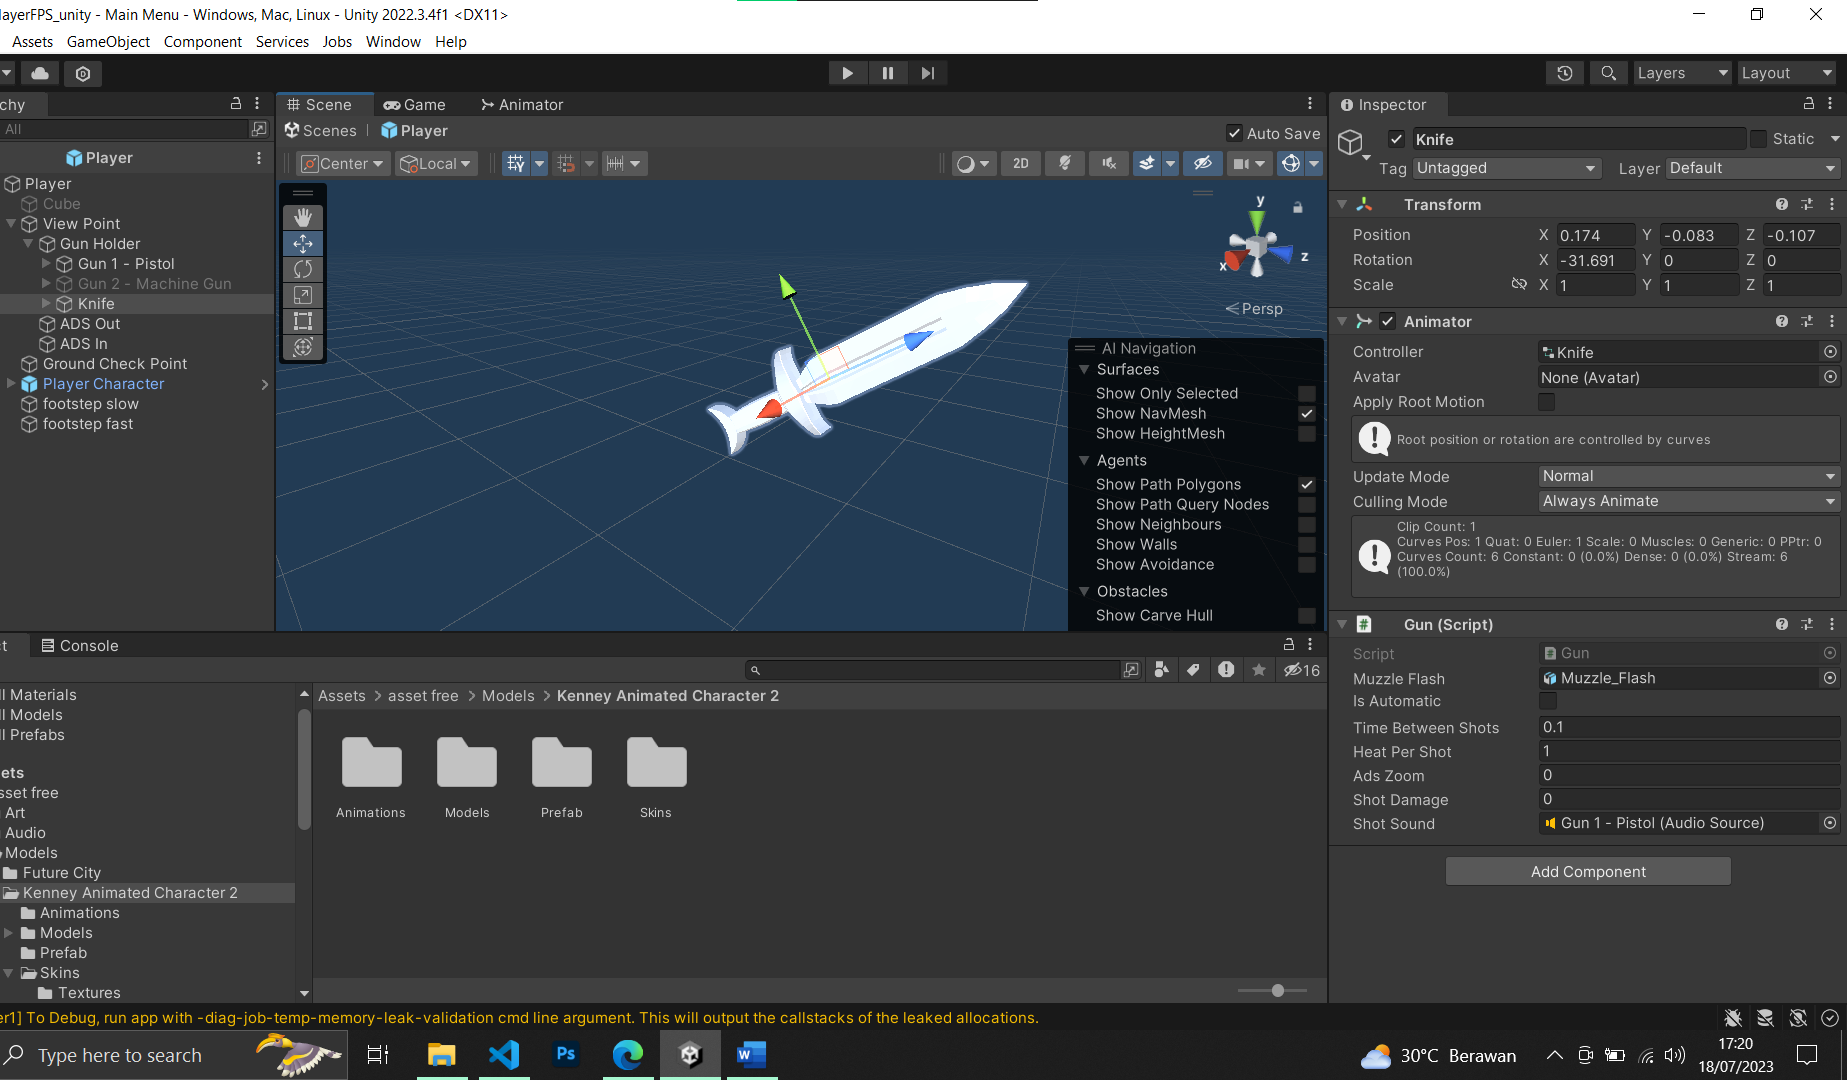
\includegraphics[width=\linewidth, height=60mm]{weapon3.png}
        \end{minipage}
        &
        \begin{minipage}{6cm}
            Knife
        \end{minipage}
        \\ \hline
        \end{tabular}
    \end{table}
\end{enumerate}

\section{Pembahasan}
\noindent

Tahap ini merupakan tahap yang berisi penjelasan bagaimana proses game ini dapat bekerja sebagaimana yang diharapkan dan dapat berjalan sesuai rancangan yang telah dibuat. Pada tahap ini meliputi Proses pembuatan game, implementasi photon, gameplay, menu, karakter dan program.

\subsection{Proses Pembuatan Game}
\begin{enumerate}
    \item Pembuatan Menu\\
    Tahap pertama adalah membuat menu dimana menu ini akan berinteraksi dengan player.
    \begin{figure}[h]
        \centering
        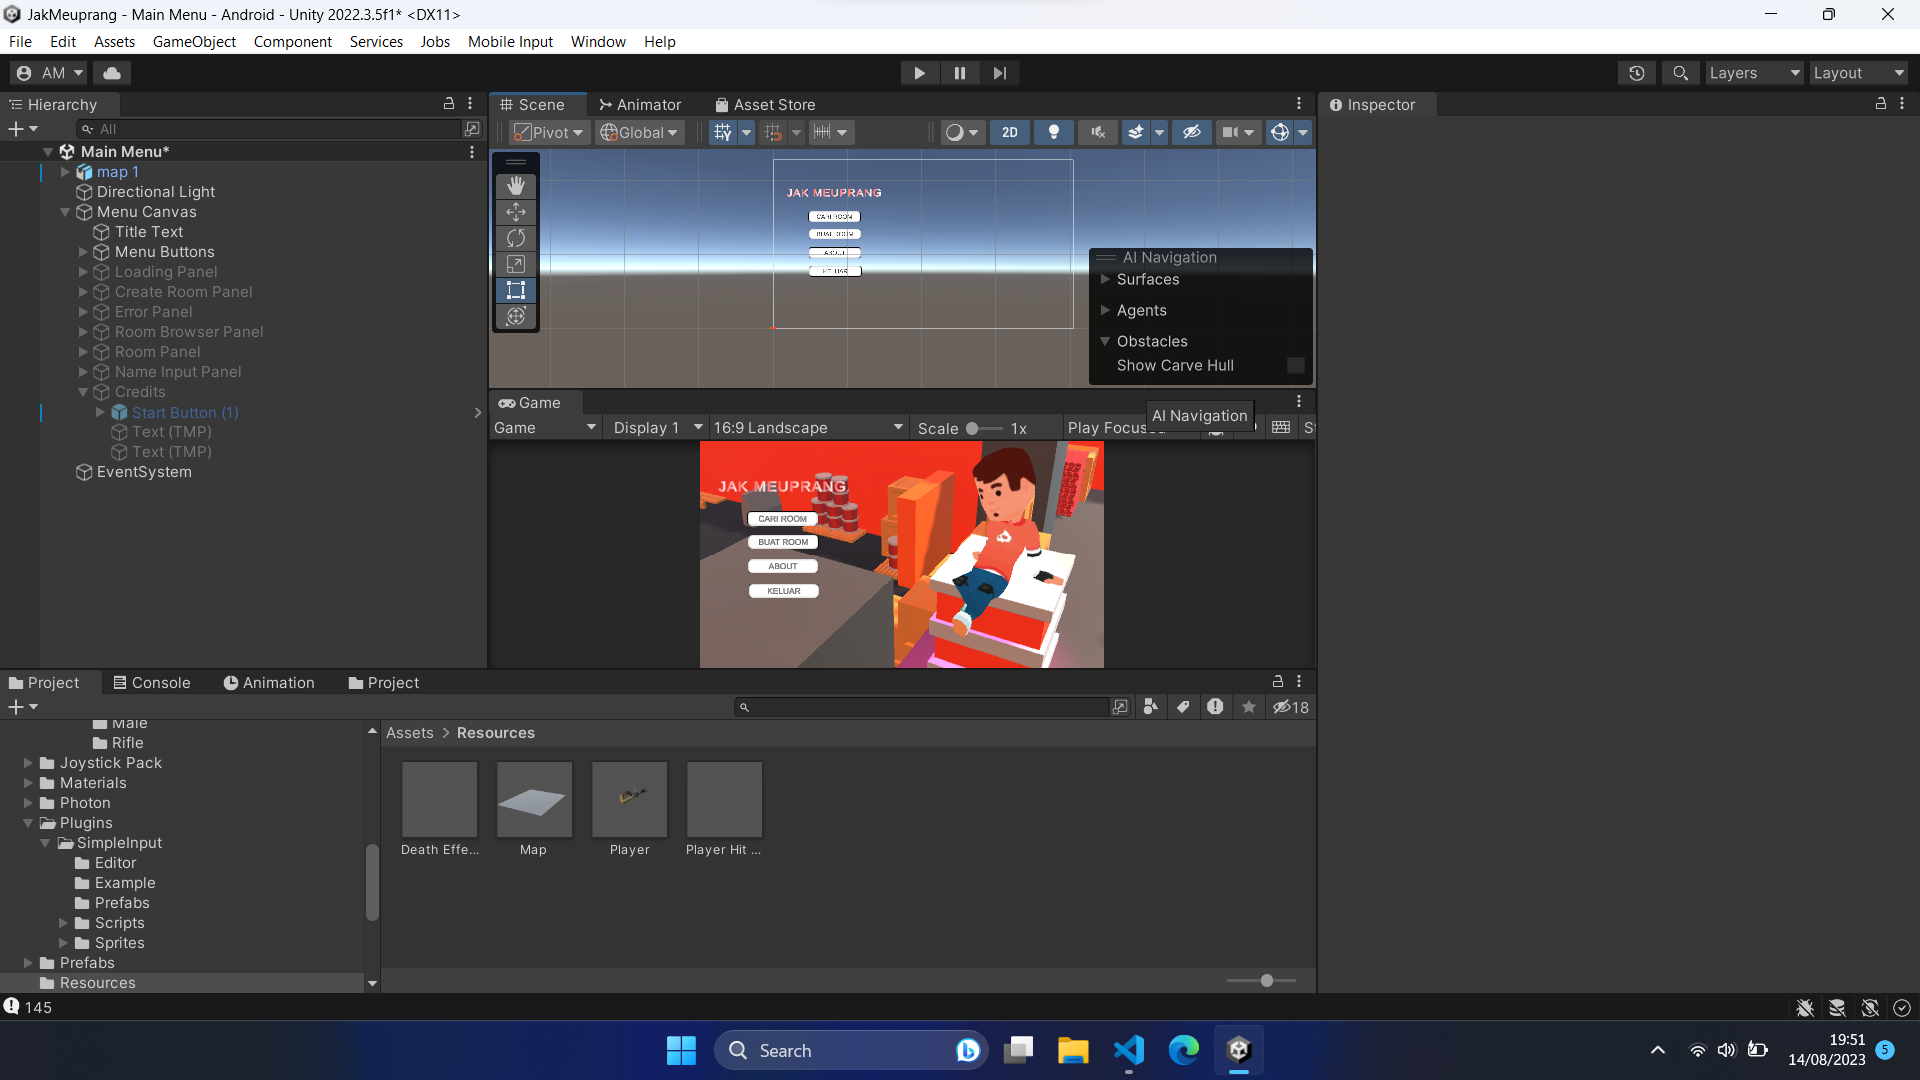
\includegraphics[width=10cm]{pembuatanmenu.png}
        \caption{Tampilan Pembuatan Menu}
        \label{fig:pembuatanmenu}
    \end{figure}
    \item Pembuatan Player Prefabs \\
    Tahap pembuatan player prefabs ini adalah untuk memberikan player dengan karakter yang disediakan menggunakan asset gratis agar dapat digunakan saat bermain.
    \newpage
    \begin{figure}[h]
        \centering
        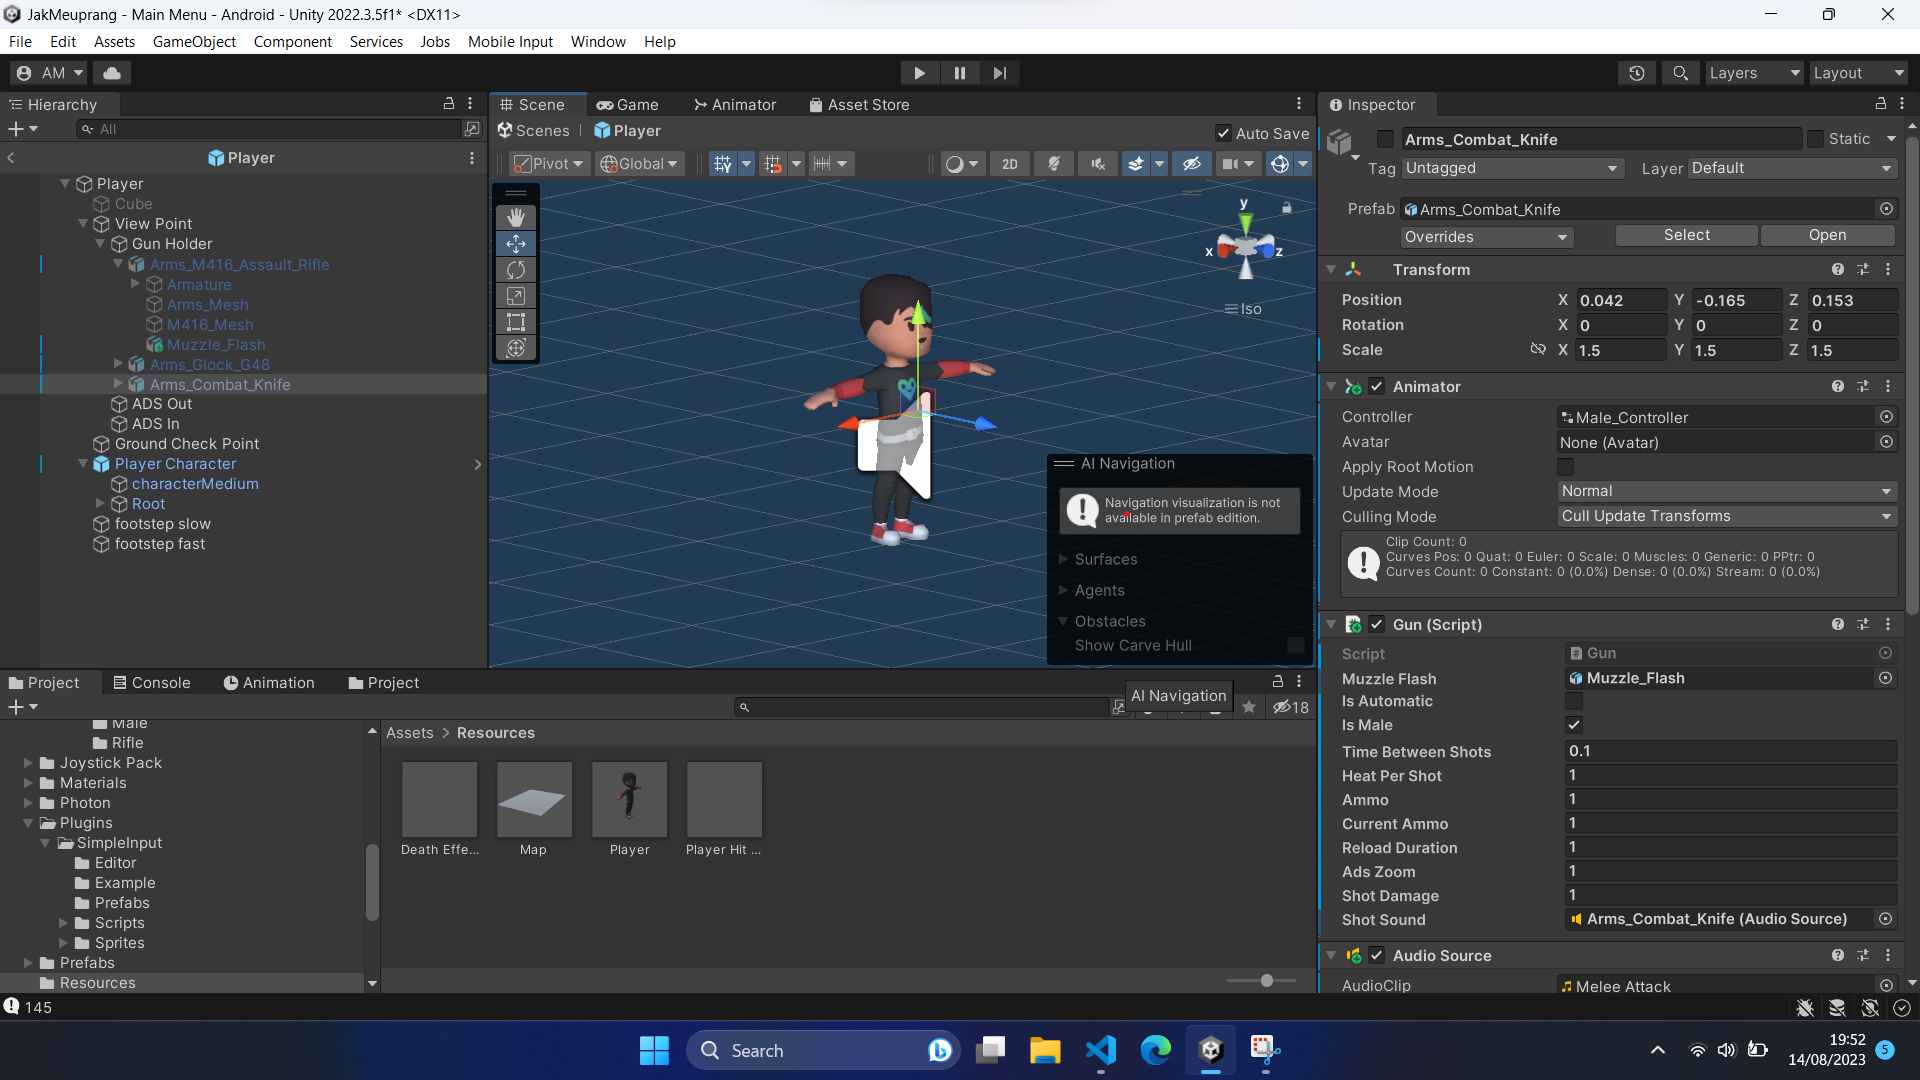
\includegraphics[width=10cm]{pembuatanplayer.png}
        \caption{Tampilan Pembuatan Player}
        \label{fig:pembuatanplayer}
    \end{figure}
    \item Pembuatan Animasi Karakter \\
    Pada tahap ini untuk membuat animasi dari karakter yang disediakan, dari gerakan idle dimana karakter berdiam, walking dimana saat karakter digerakan akan ada animasi berjalan, dan berlari jika inputan dari user terdeteksi berlari akan melakukan animasi berlari.
    \begin{figure}[h]
        \centering
        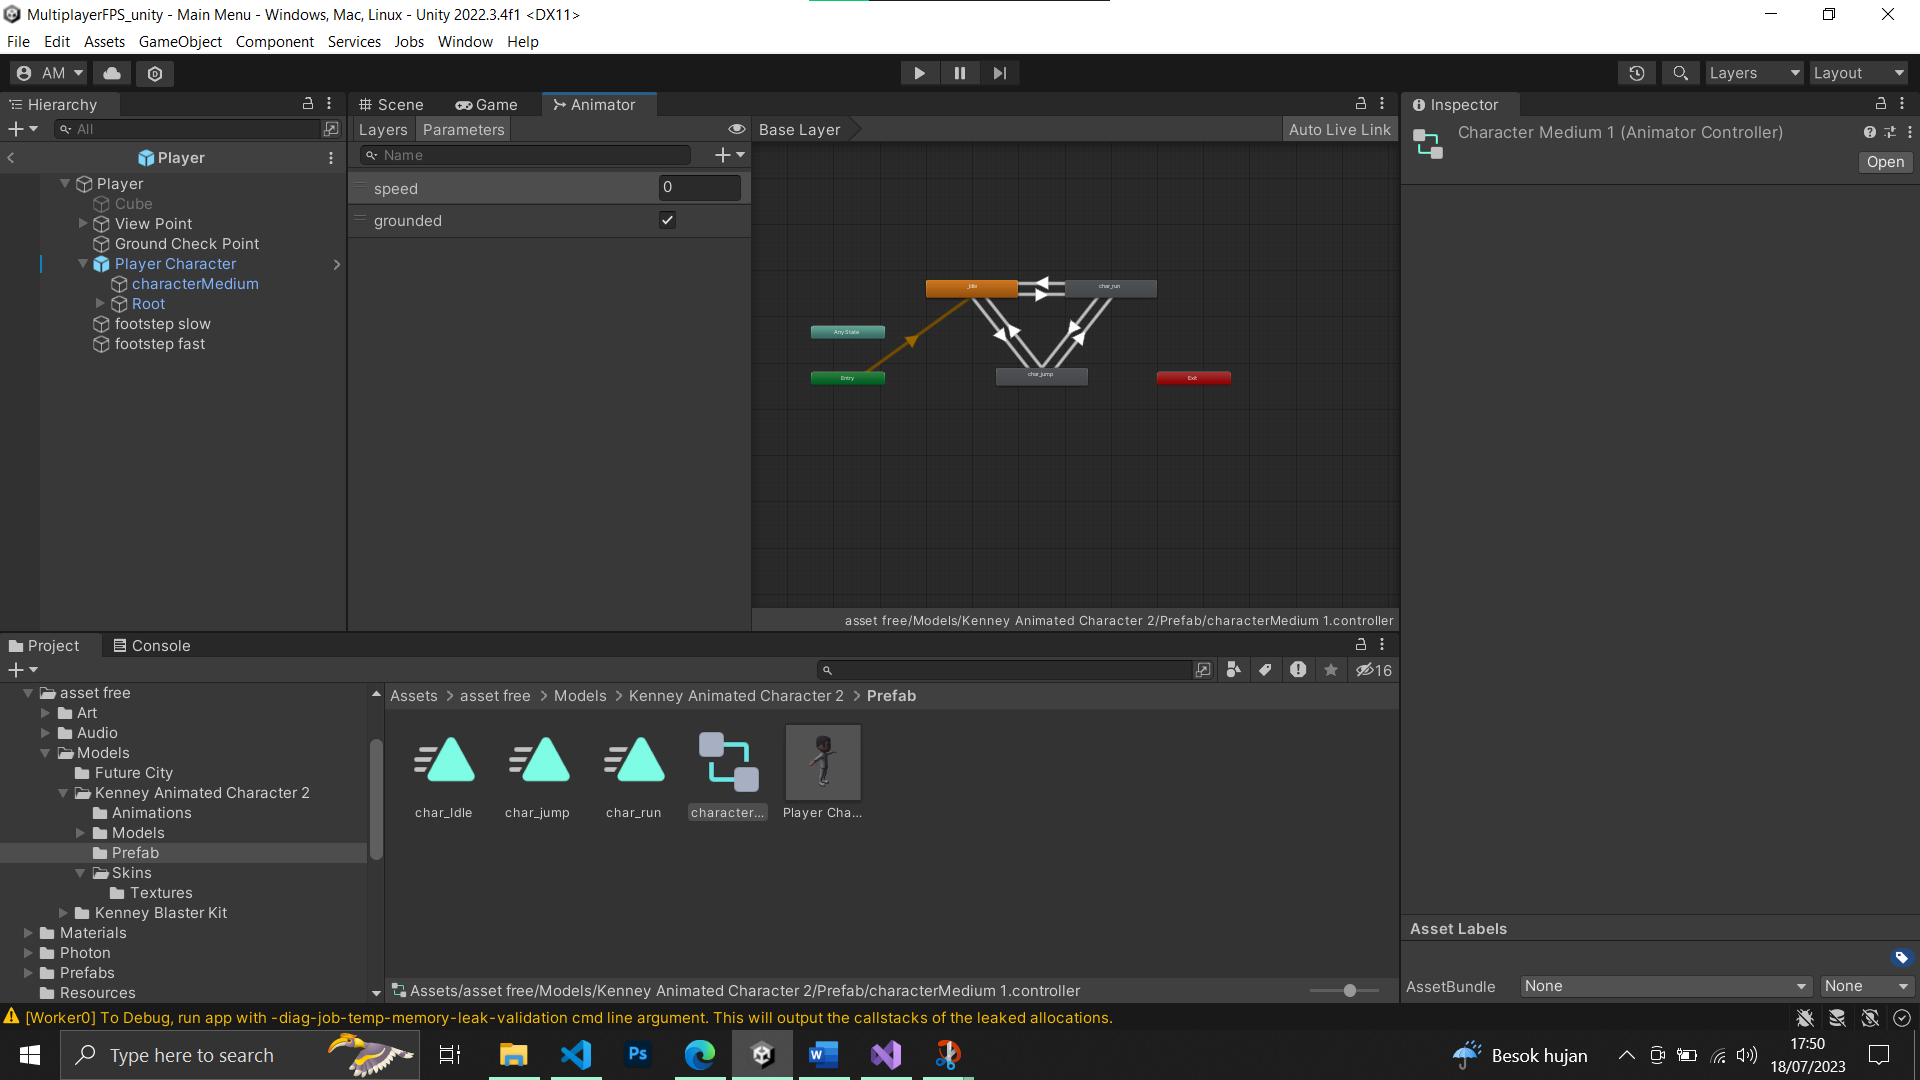
\includegraphics[width=10cm]{pembuatananimasi.png}
        \caption{Tampilan Pembuatan Animasi}
        \label{fig:pembuatananimasi}
    \end{figure}
    \item Objek didalam game \\ 
    Pada tahap ini menjelaskan objek objek yang terdapat saat didalam permainan
    \begin{enumerate}
        \item Weapon\\
        Player mendapatkan 3 senjata yaitu pistol, rifle, pisau.
        \item Health \\
        Player diberikan darah , jika darah berkurang makan player akan terdestroy objectnya.
        \item Weapon Overheat \\
        Player diberikan batas saat menembak, jika melebihi batas tersebut maka senjata tersebut akan overheat.
    \end{enumerate}
    \item Sound \\
    Pada tahap ini memberikan sound pada beberapa object yaitu :
    \begin{enumerate}
        \item Backsound \\
        Memberikan sound saat dalam main menu.
        \item Foot Step Low \\ 
        Memberikan sound saat player sedang berjalan maka menggunakan sound foot step low.
        \item Foot Step Fast \\
        Memberikan sound saat player berlari maka menggunakan sound foot step fast.
        \item Memberikan Sound Senjata \\ 
        Dengan memberikan sound masing masing pada senjata yang digunakan.
    \end{enumerate}
\end{enumerate}

\subsection{Map Gameplay}
Tahap ini adalah tahap pembuatan map yang digunakan saat bermain, map ini menggunakan asset low poly yang diberikan secara gratis dan dimplementasikan
\begin{figure}[h]
    \centering
    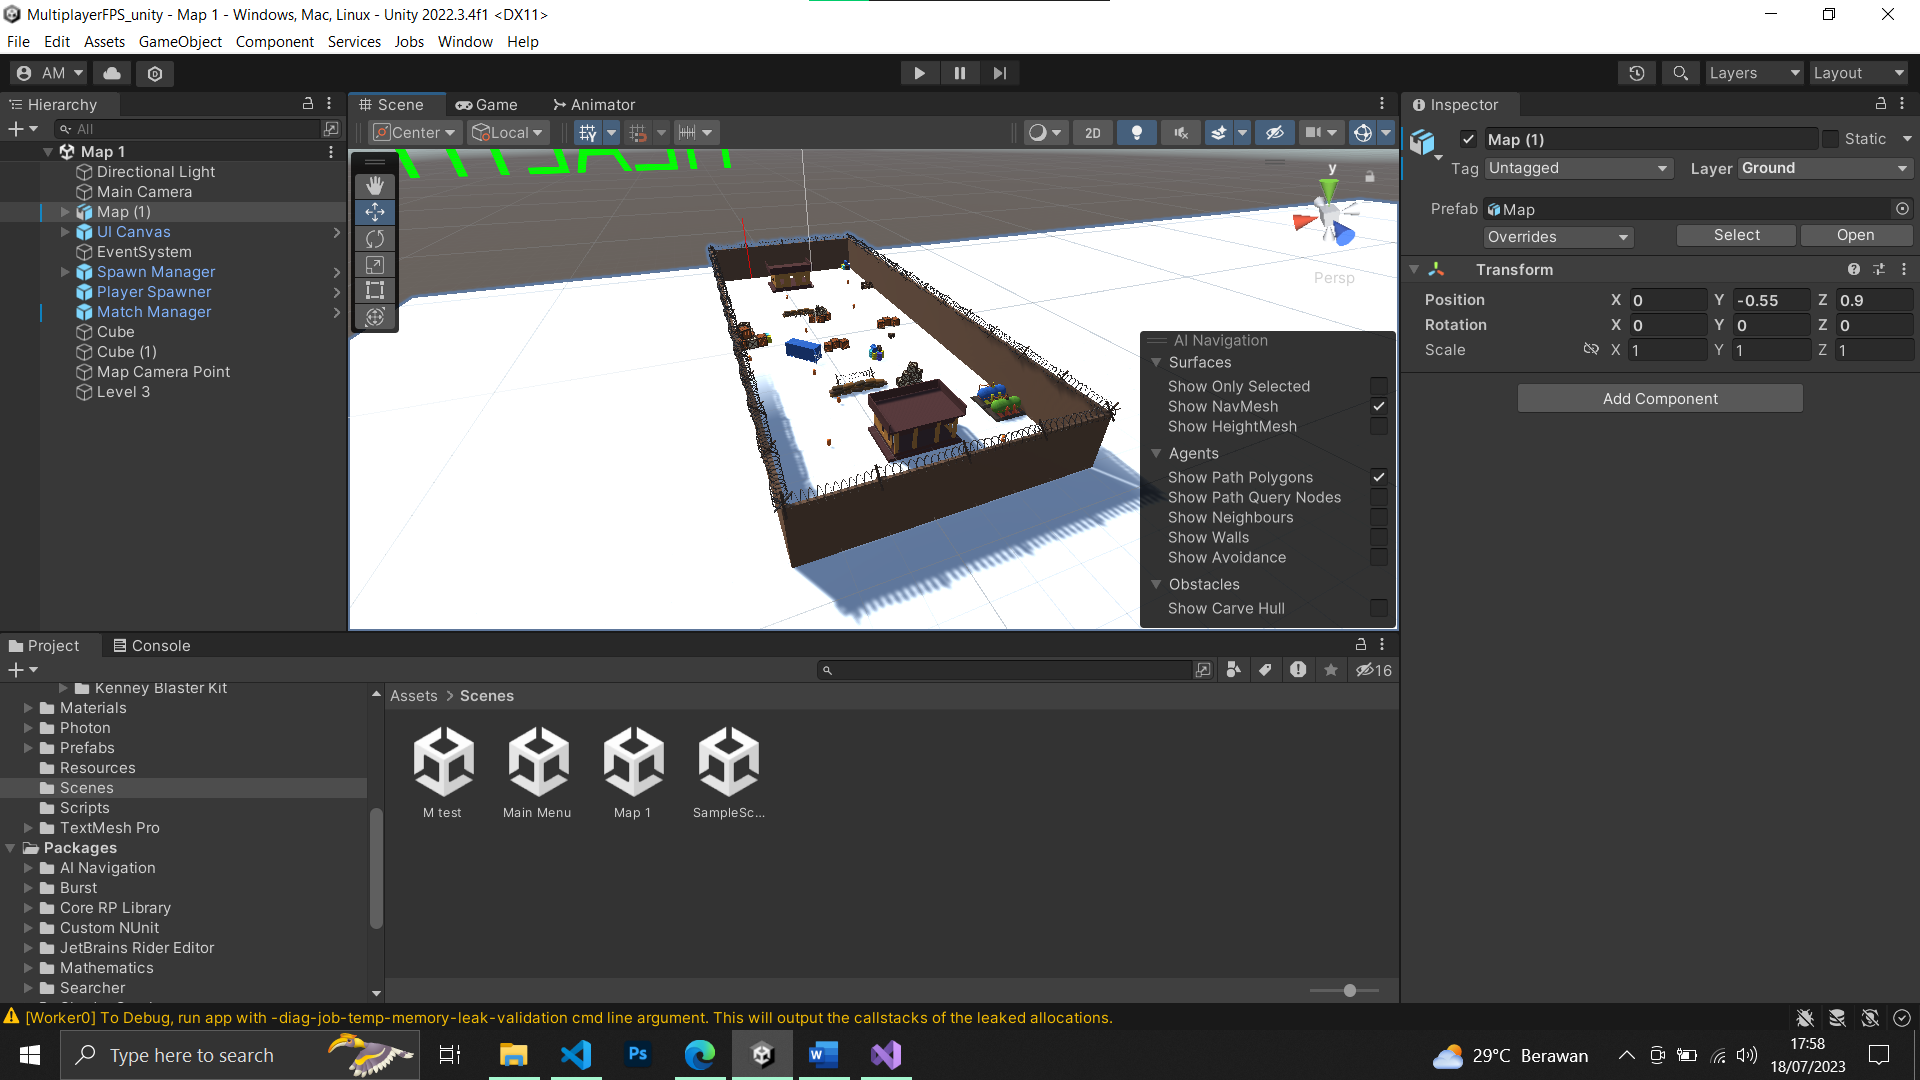
\includegraphics[width=10cm]{pembuatanmap.png}
    \caption{Tampilan Pembuatan Map}
    \label{fig:pembuatanmap}
\end{figure}

\newpage
\subsection{Program}
\noindent

Pada bagian ini akan menampilkan source code yang akan menjalankan dari interaksi interkasi object object yang telah dibuat seperti berjalan, menembak, memasuki room dan lainnya.

\begin{enumerate}
    \item Implementasi Server Photon \\
    Code ini berfungsi untuk melakukan connecting ke server photon, dengan menutup menu lainnya terlebih dahulu, jika server sudah terkoneksi maka akan masuk kedalam instance set nama dan menu.
    \begin{figure}[h]
        \centering
        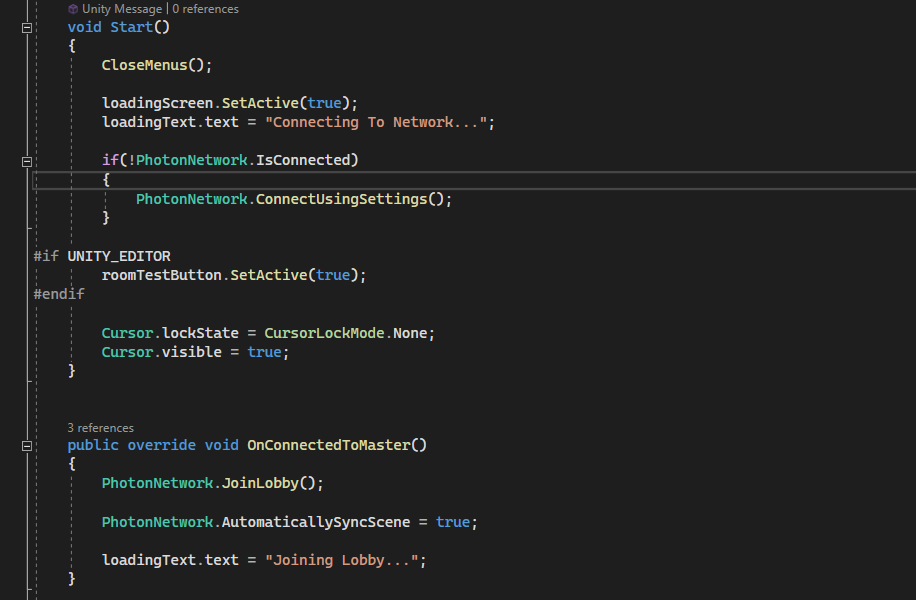
\includegraphics[width=10cm]{implementasiphoton.png}
        \caption{Tampilan Code Photon}
        \label{fig:connectingp}
    \end{figure}
    \item \textit{Source Code} Create Room \\
    Pada code ini berfungsi untuk melakukan pembuatan room dengan memberikan nama room, max player, dan memanggil photonetwork untuk melakukan pembuatan room.
    \newpage
    \begin{figure}[h]
        \centering
        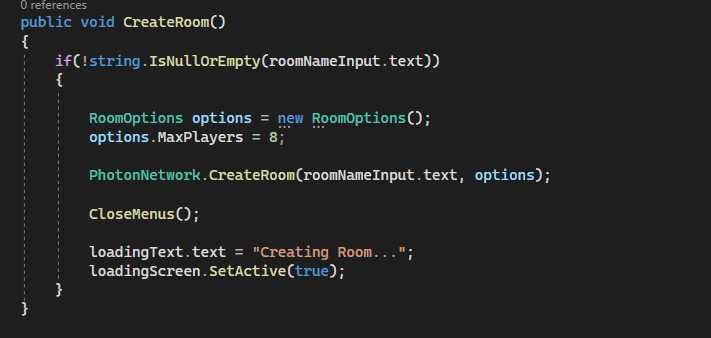
\includegraphics[width=10cm]{codepembuatanroom.png}
        \caption{Tampilan Code Pembuatan Room}
        \label{fig:pembuatanroom}
    \end{figure}
    \item \textit{Source Code Joinned Room} \\
    Code ini berfungsi untuk memberikan instance jika player join room akan menampikan room yang dimasuk dengan player player yang tersedia pada room tersebut.
    \begin{figure}[h]
        \centering
        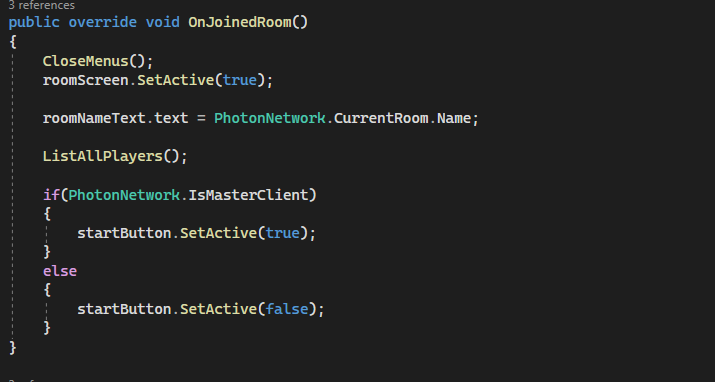
\includegraphics[width=10cm]{joinnedroom.png}
        \caption{Tampilan Code Joinned Room}
        \label{fig:joinnedroom}
    \end{figure}
    \item \textit{Source Code Start Game}\\
    Code ini berfungsi untuk melakukan pemindahan instance ke scene map jika player memulai room yang telah dibuat.
    \begin{figure}[h]
        \centering
        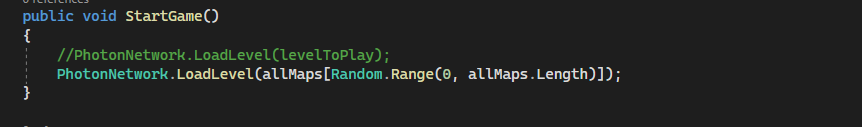
\includegraphics[width=10cm]{startgame.png}
        \caption{Tampilan Code Start Game}
        \label{fig:startgame}
    \end{figure}
    \newpage
    \item \textit{Source Code Player Controller} \\
    Code ini berfungsi untuk memberikan instance pertama player respawn saat dimainkan
    \begin{figure}[h]
        \centering
        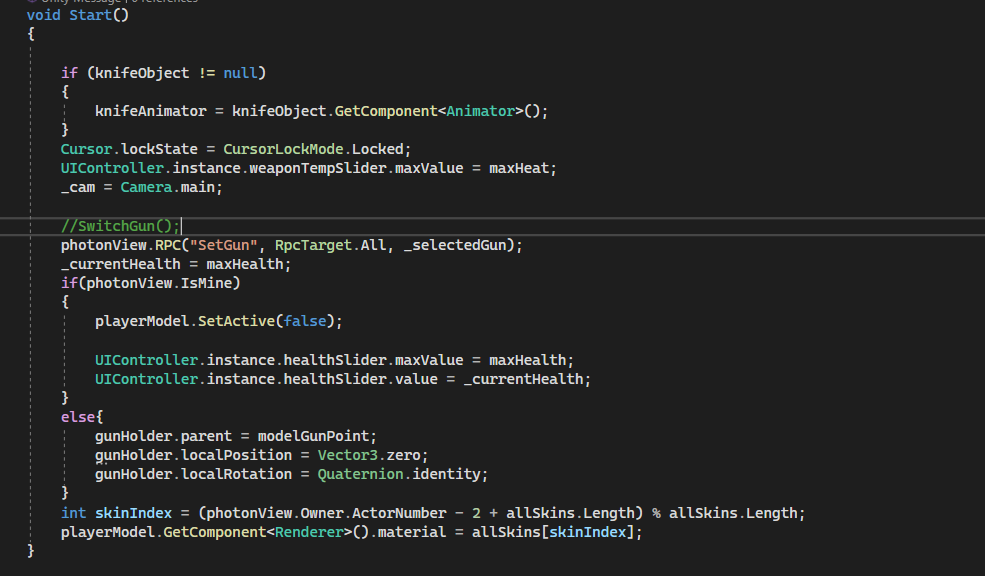
\includegraphics[width=10cm]{playerinstance.png}
        \caption{Tampilan Code Player Instance}
        \label{fig:playerinstance}
    \end{figure}
    \item \textit{Source Code Switch Gun} \\ 
    Code ini berfungsi untuk melakukan pergantian senjata pada player.
    \begin{figure}[h]
        \centering
        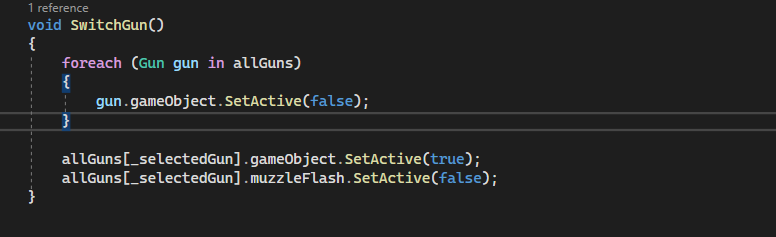
\includegraphics[width=10cm]{switchgun.png}
        \caption{Tampilan Code Switch}
        \label{fig:switchgun}
    \end{figure}
    \item \textit{Source Code Damage} \\
    Code ini berfungsi menerima damage pada player.
    \newpage
    \begin{figure}[h]
        \centering
        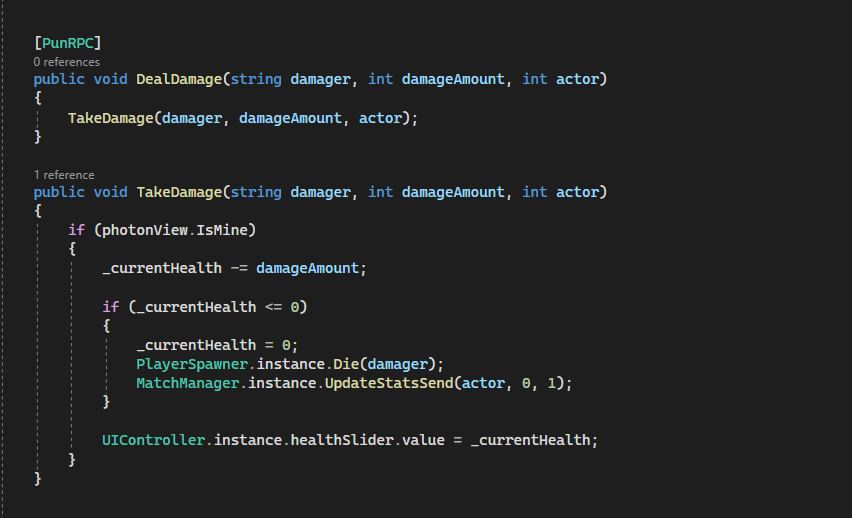
\includegraphics[width=10cm]{takedamage.png}
        \caption{Tampilan Code Take Damage}
        \label{fig:takedamage}
    \end{figure}
    \item \textit{Source Code Shoot} \\ 
    Code ini berfungsi untuk membuat player tembakan.
    \begin{figure}[h]
        \centering
        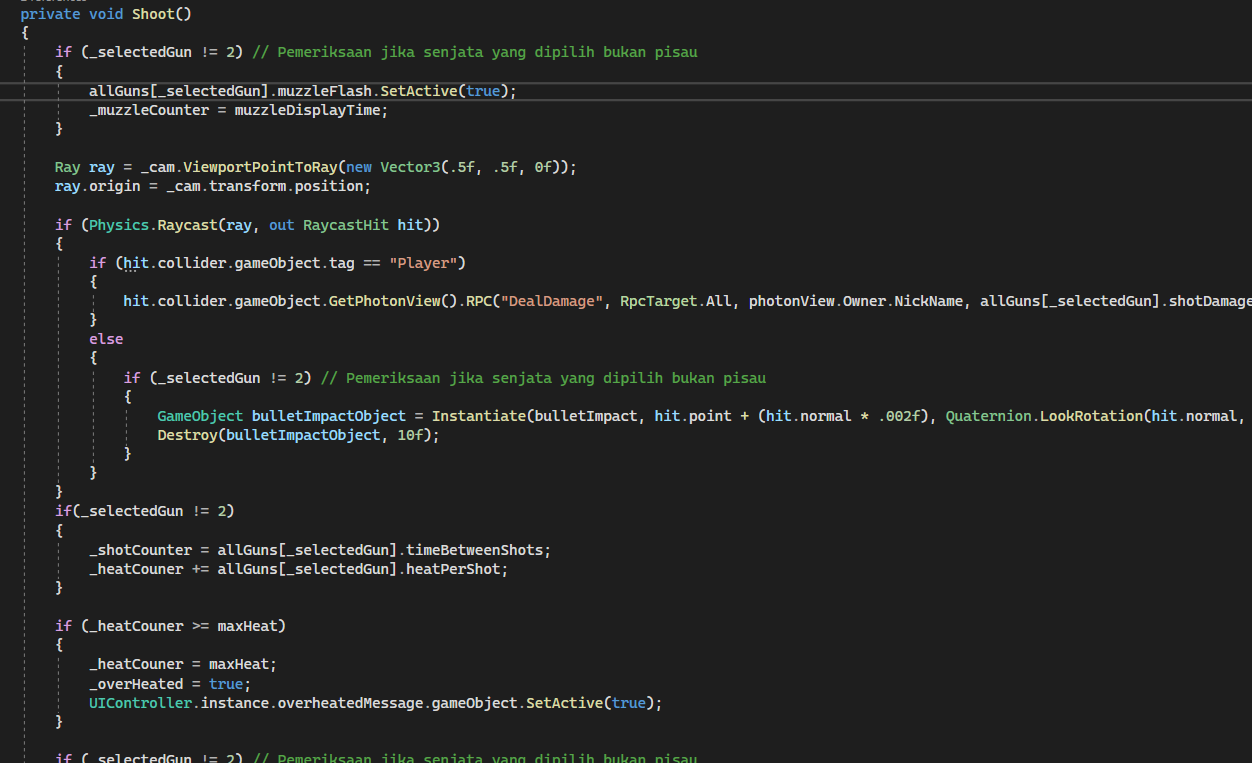
\includegraphics[width=10cm]{shoot.png}
        \caption{Tampilan Code Shoot}
        \label{fig:shoot}
    \end{figure}
    \newpage
    \item \textit{Source Code Knife} \\ 
    Code ini berfungsi untuk membuat player memberikan animasi \textit{Knife}.
    \begin{figure}[h]
        \centering
        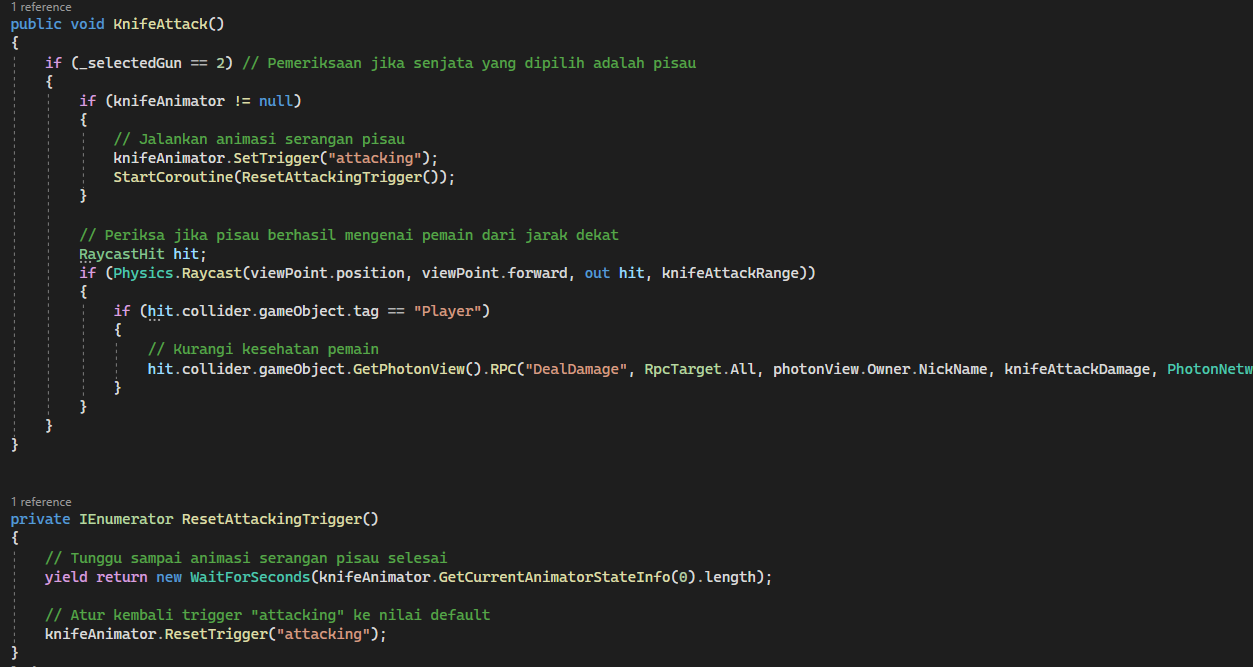
\includegraphics[width=10cm]{knife.png}
        \caption{Tampilan Code Knife}
        \label{fig:knife}
    \end{figure}
    \item \textit{Source Code Movement Player} \\ 
    Code ini Berfungsi untuk membuat bergerakan player yang didapat dari inputan.
    \begin{figure}[h]
        \centering
        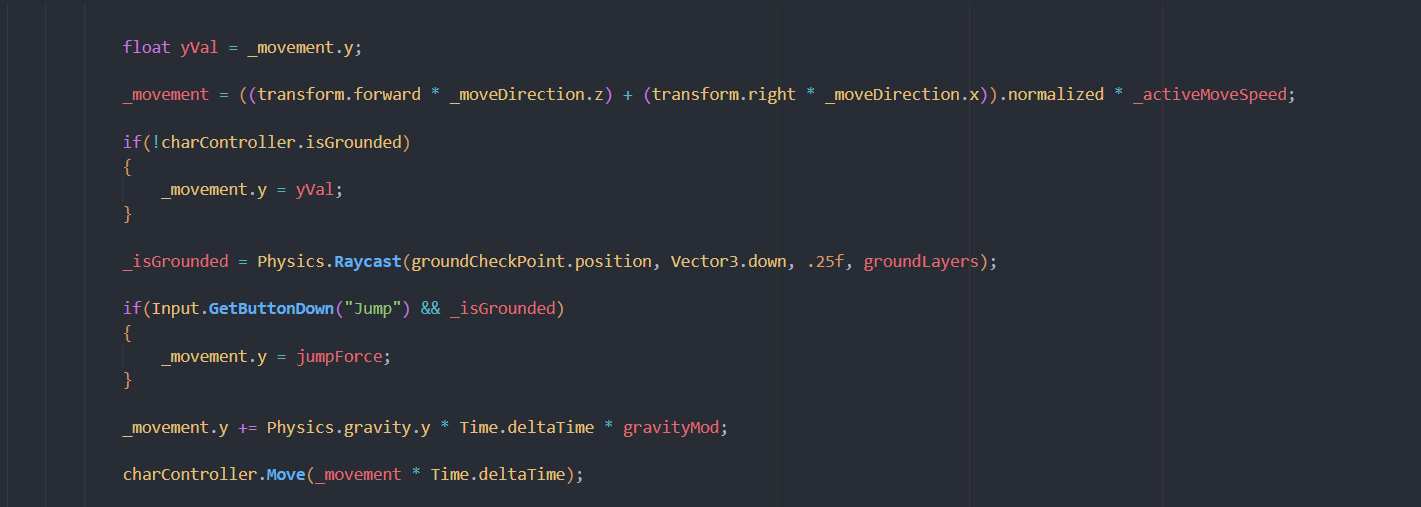
\includegraphics[width=10cm]{player-movement.png}
        \caption{Tampilan Code Player Movement}
        \label{fig:movementp}
    \end{figure}
    \item \textit{Source Code Match Manager} \\
    Code ini berfungsi untuk melakukan instance match manager untuk mengatur logika selama bermain.
    \newpage
    \begin{figure}[h]
        \centering
        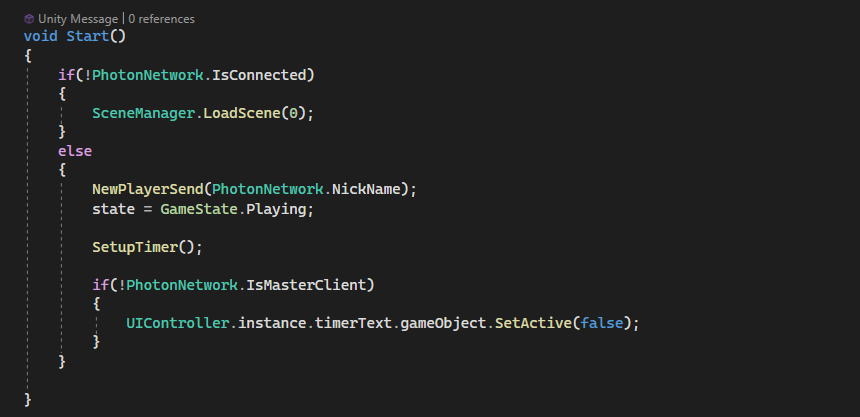
\includegraphics[width=10cm]{matchmanager.png}
        \caption{Tampilan Code Match Manger}
        \label{fig:matchmanager}
    \end{figure}
    \item \textit{Source Code Leaderboard} \\ 
    Code ini berfungsi untuk menampilkan leaderboard saat bermain.
    \begin{figure}[h]
        \centering
        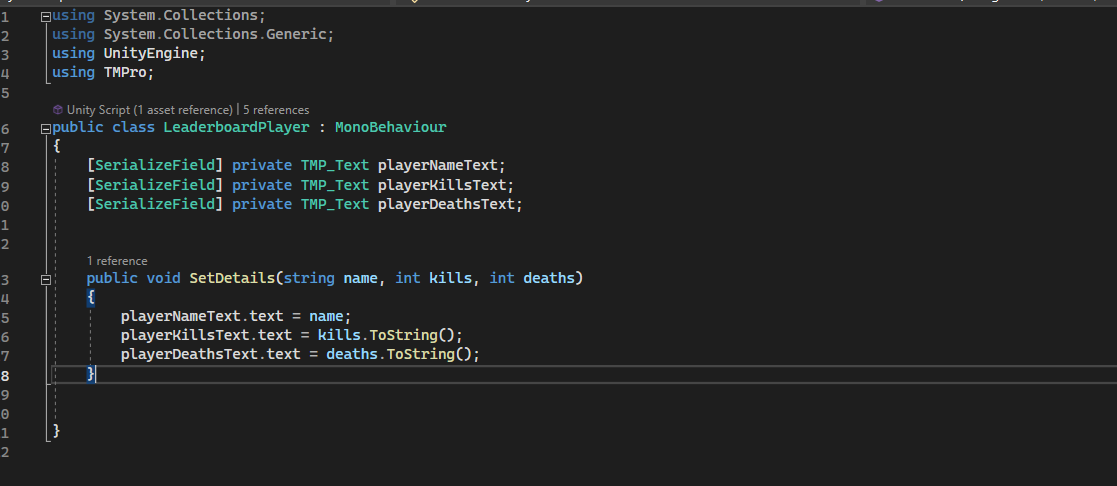
\includegraphics[width=10cm]{leaderboard.png}
        \caption{Tampilan Code LeaderBoard}
        \label{fig:leaderboard}
    \end{figure}
    \item \textit{Source Code Spawn Manager}\\
    Code ini berfungsi untuk memberikan spawn player secara random dengan titik yang telah ditentukan.
   \newpage
    \begin{figure}[h]
        \centering
        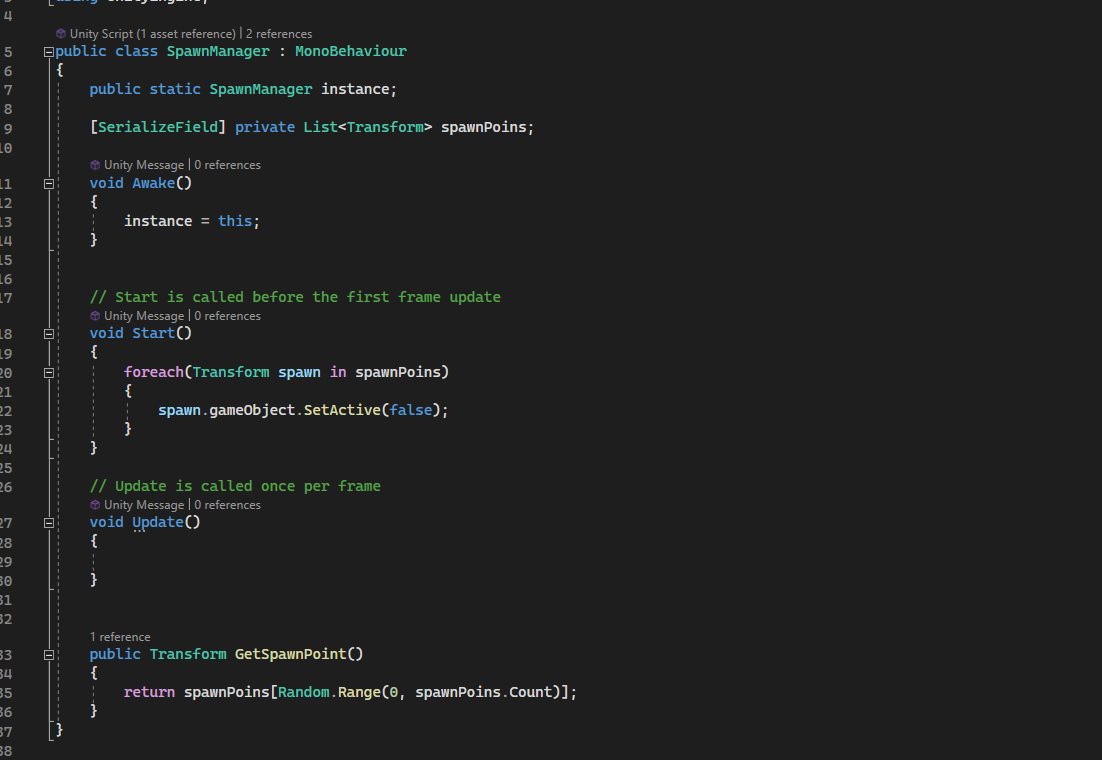
\includegraphics[width=10cm]{spawnmanager.png}
        \caption{Tampilan Code Spawn Manager}
        \label{fig:spawnmanager}
    \end{figure}
    \item \textit{Source Code Player Spawner} \\ 
    Code ini berfungsi untuk melakukan instance spawn dan matinya player.
    \begin{figure}[h]
        \centering
        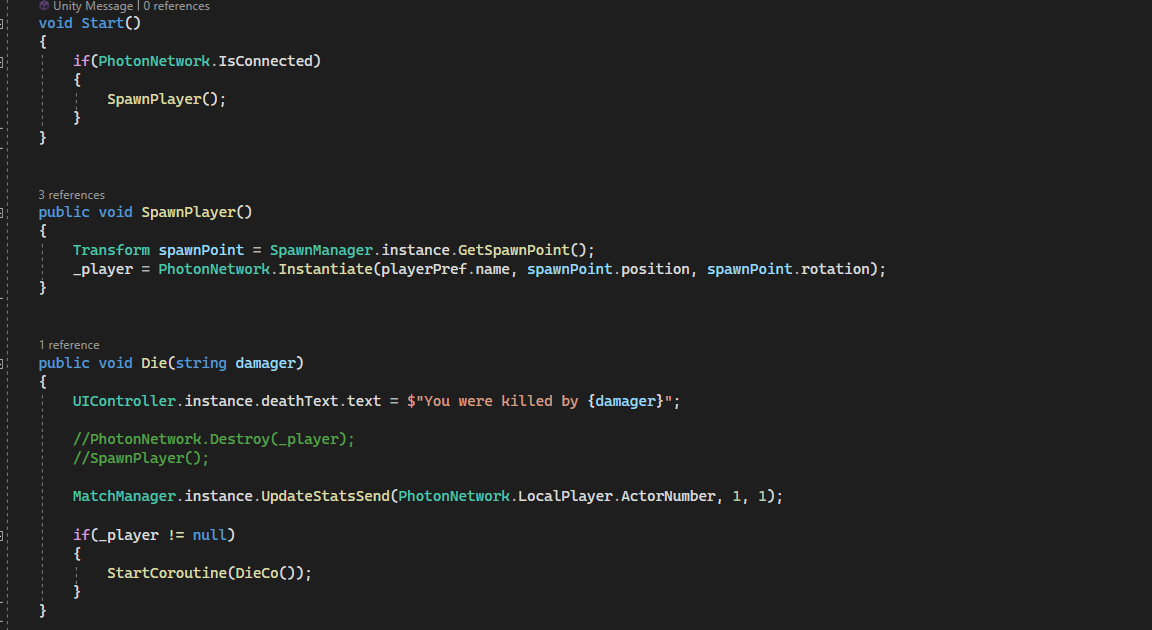
\includegraphics[width=10cm]{playerspawner.png}
        \caption{Tampilan Code Player Spawner}
        \label{fig:playerspawner}
    \end{figure}
    \item \textit{Source Code Gun} \\ 
    Code ini berfungsi untuk memberikan algoritma pada senajata yang digunakan.
    \newpage
    \begin{figure}[h]
        \centering
        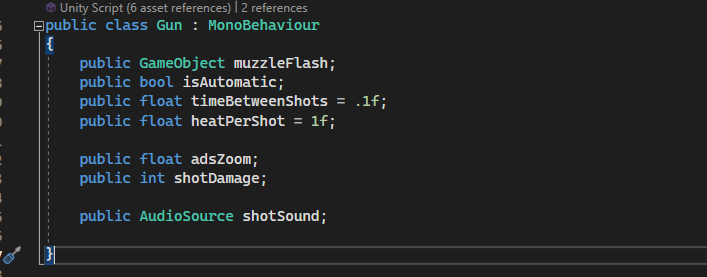
\includegraphics[width=10cm]{gun.png}
        \caption{Tampilan Code Gun}
        \label{fig:gun}
    \end{figure}
\end{enumerate}

\section{Pengujian Multiplayer Online}

Pada pengujian multiplayer online ini terdapat 5 player untuk melakukan pengujian secara online dengan jaringan yang berbeda.
\begin{enumerate}
    \item Pengujian Mencari room \\
    Pada Pengujian ini player pertama mencari room yang dibuat oleh player kedua, dan pada pengujian pencarian room ini berhasil seperti gambar \ref{fig:pencarianroom}. 
    \begin{figure}[h]
        \centering
        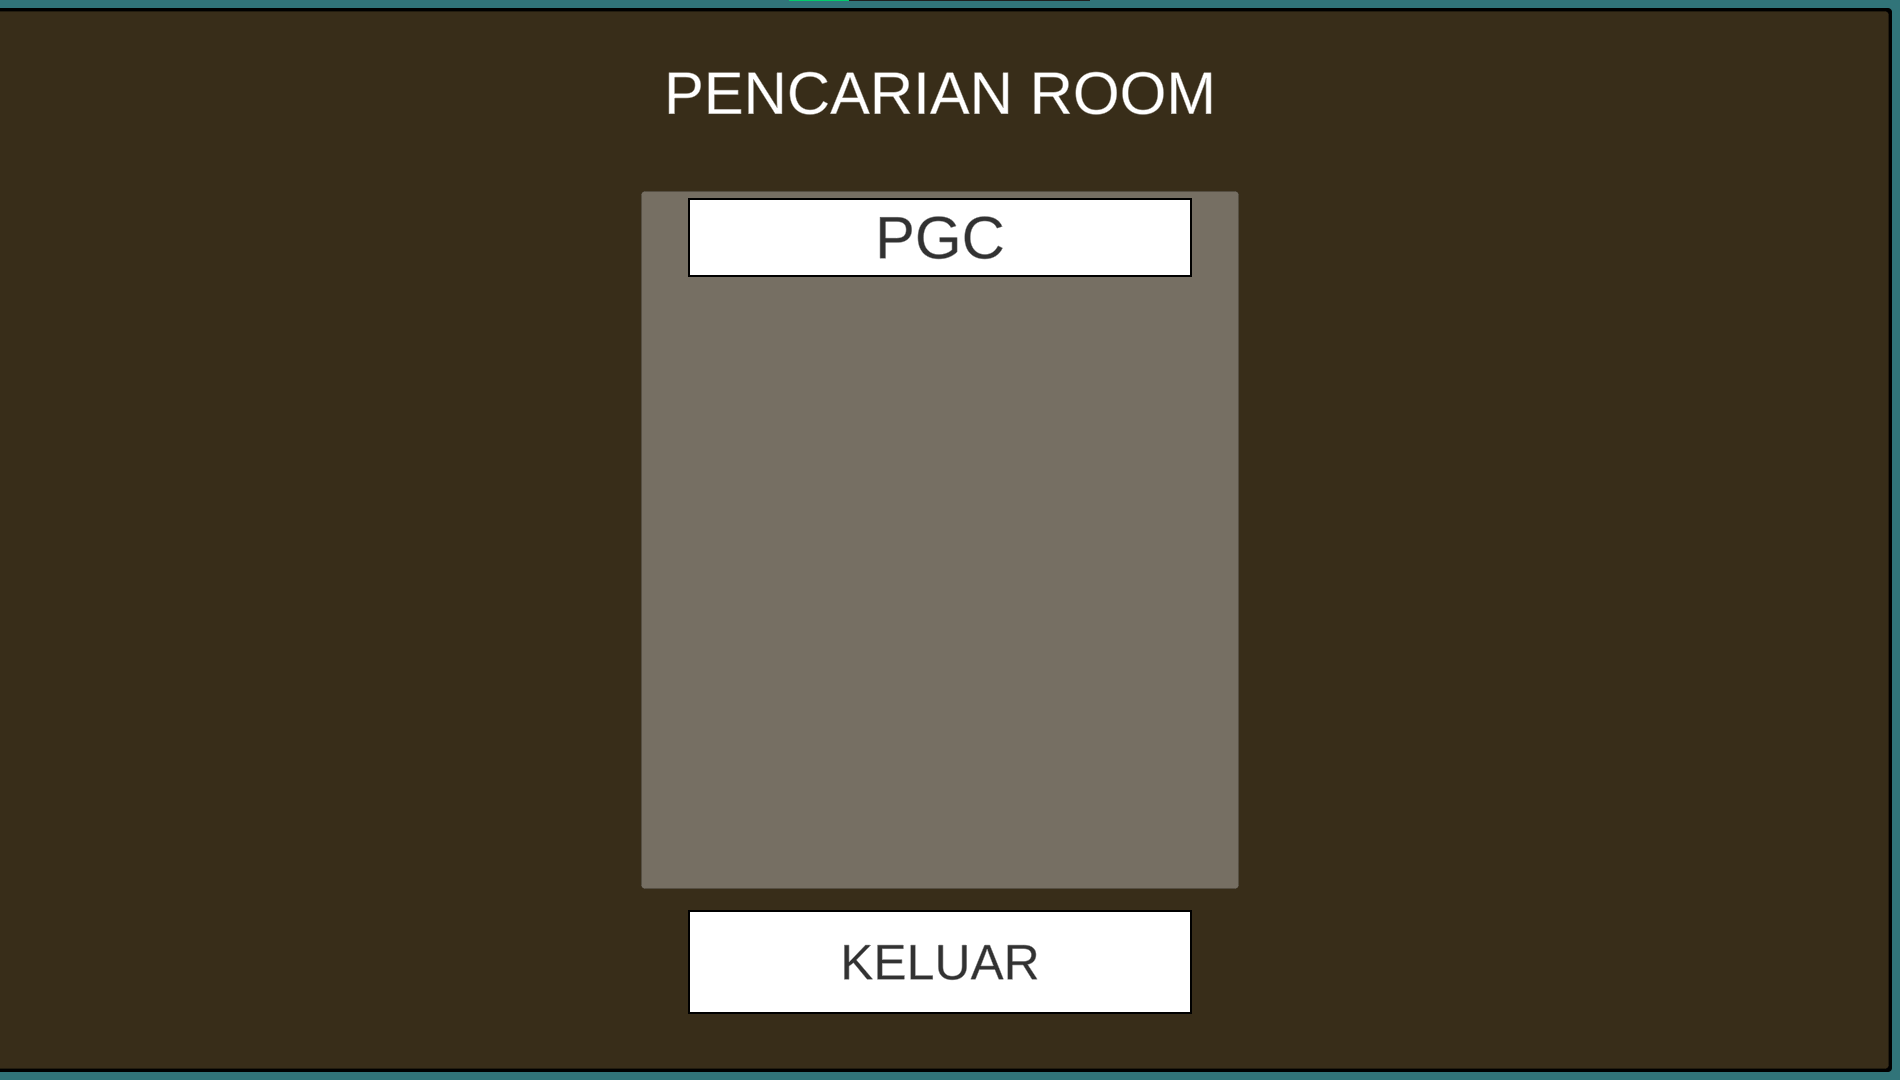
\includegraphics[width=10cm]{pencarianroom.png}
        \caption{Tampilan Pencarian Room}
        \label{fig:pencarianroom}
    \end{figure}
    \item Pengujian Masuk Room \\
    Pada Pengujian memasuki room player berhasil menjumpai sesama player didalam room tersebut seperti gambar \ref{fig:didalamroom}.
    \newpage
    \begin{figure}[h]
        \centering
        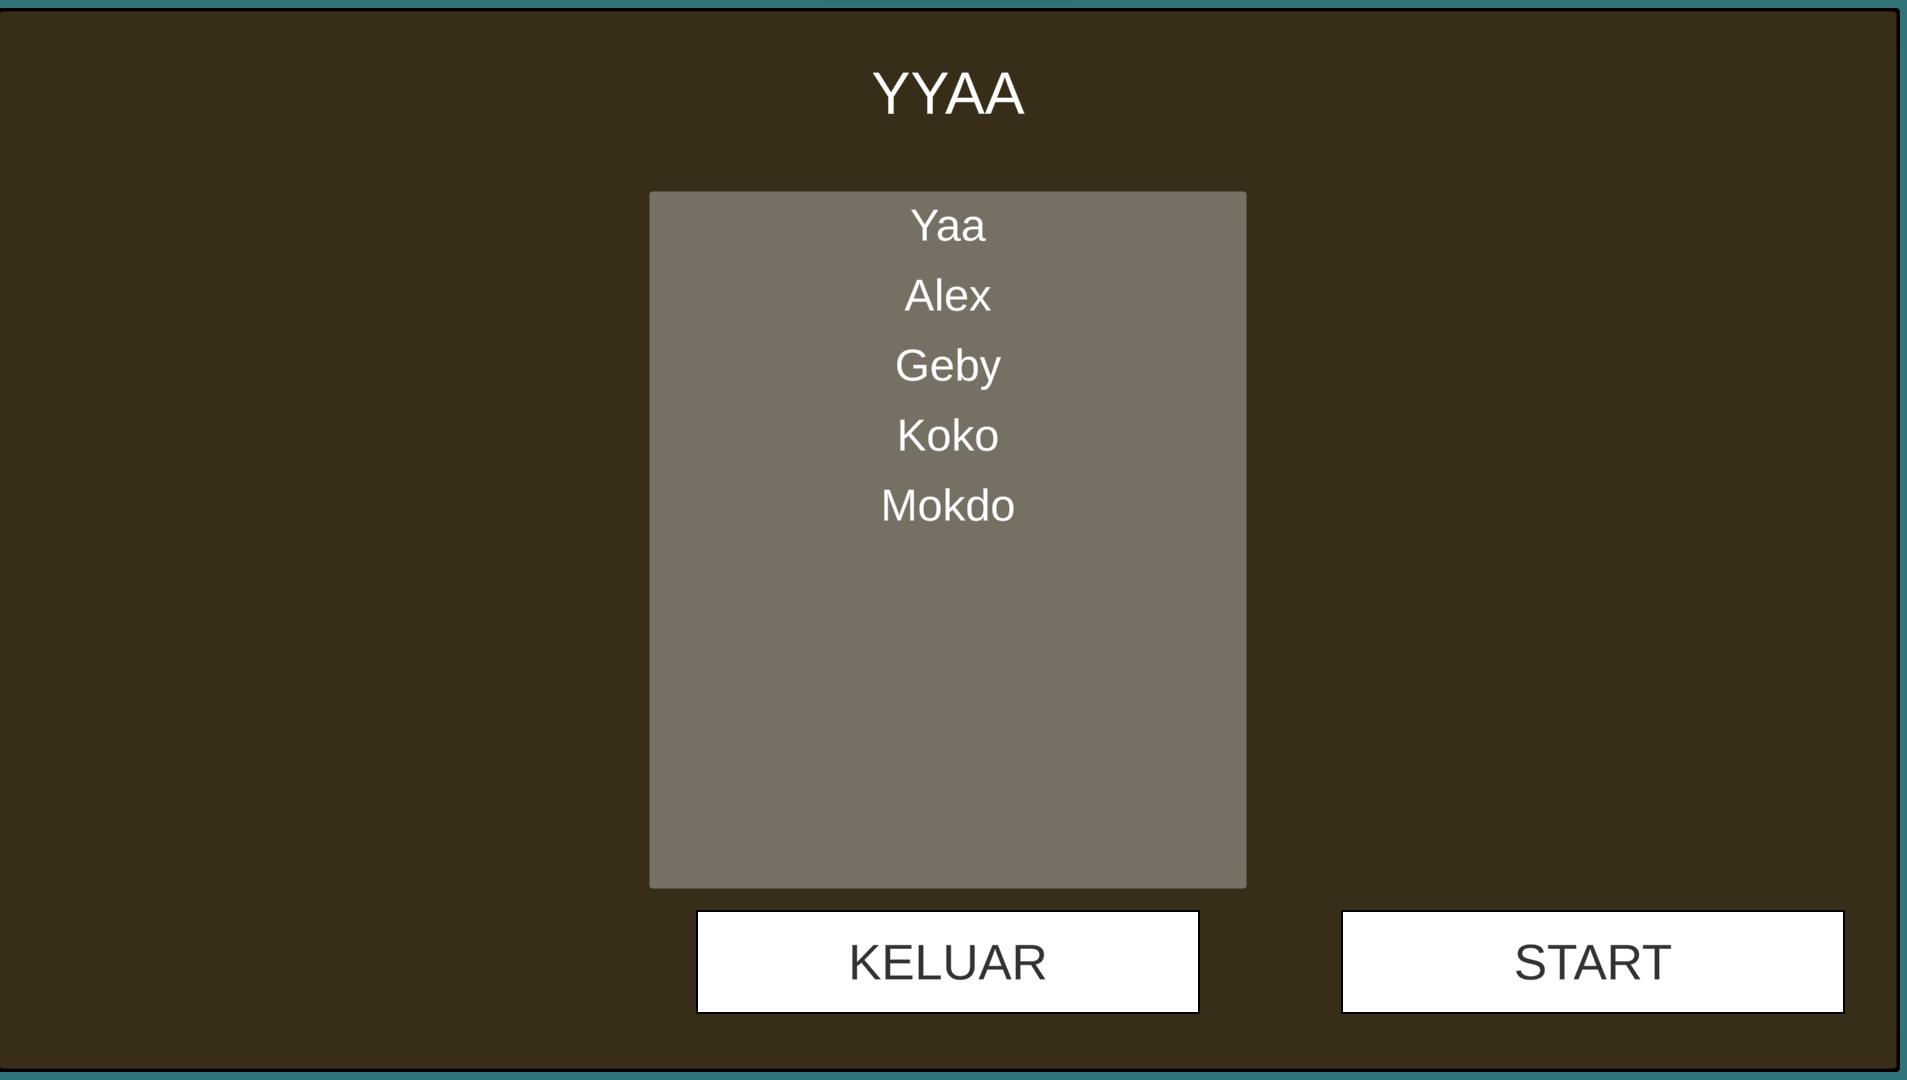
\includegraphics[width=10cm]{5-player.png}
        \caption{Tampilan Didalam Room}
        \label{fig:didalamroom}
    \end{figure}
    \item Pengujian Mulai Game \\
    Pada Pengujian mulai game, player berhasil menjumpai sesama player didalam instance game secara online.
    \begin{figure}[h]
        \centering
        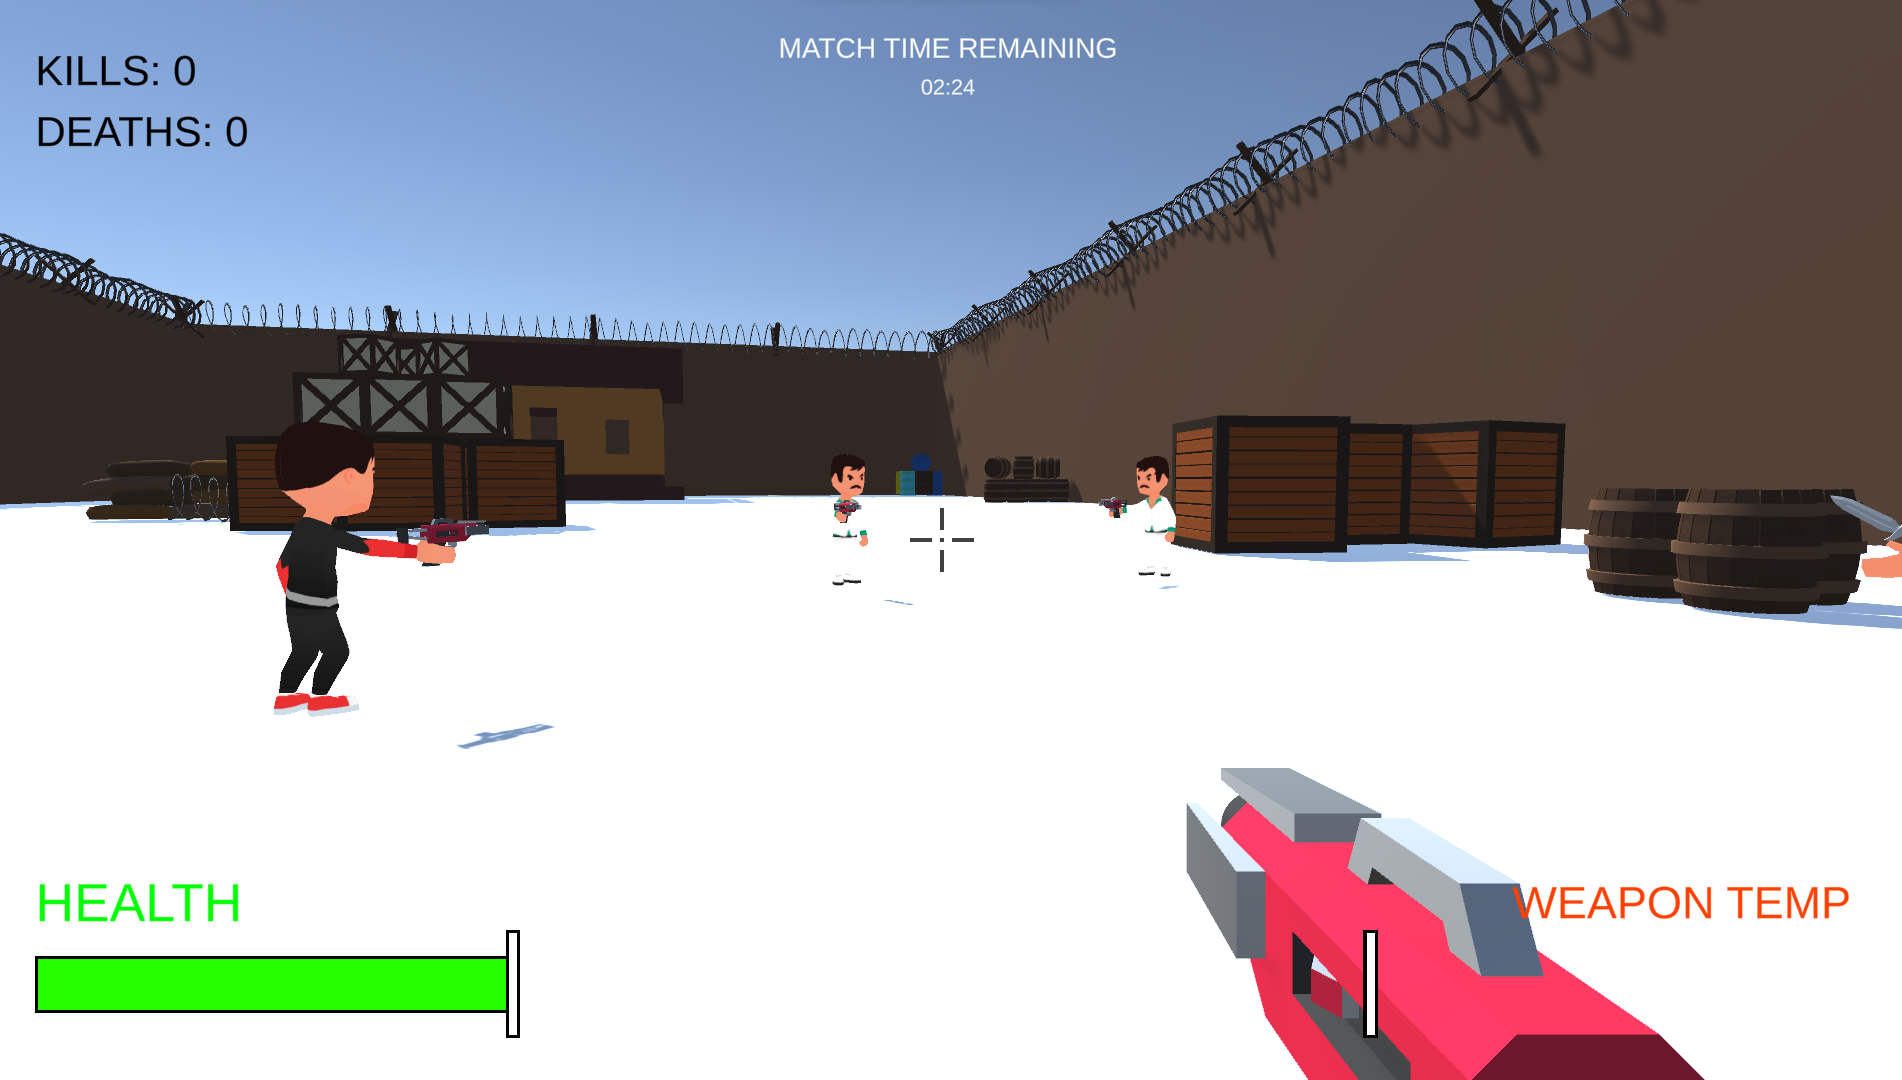
\includegraphics[width=10cm]{5-player-ingame.png}
        \caption{Tampilan Dalam Game}
        \label{fig:dalamgame}
    \end{figure}
    \item Pengujian \textit{Battle} \\
    Pada pengujian ini player melakukan peperangan untuk mencari point, pengujian ini berhasil dikarenakan player mati saat ditembaki oleh player lain.
    \newpage
    \begin{figure}[h]
        \centering
        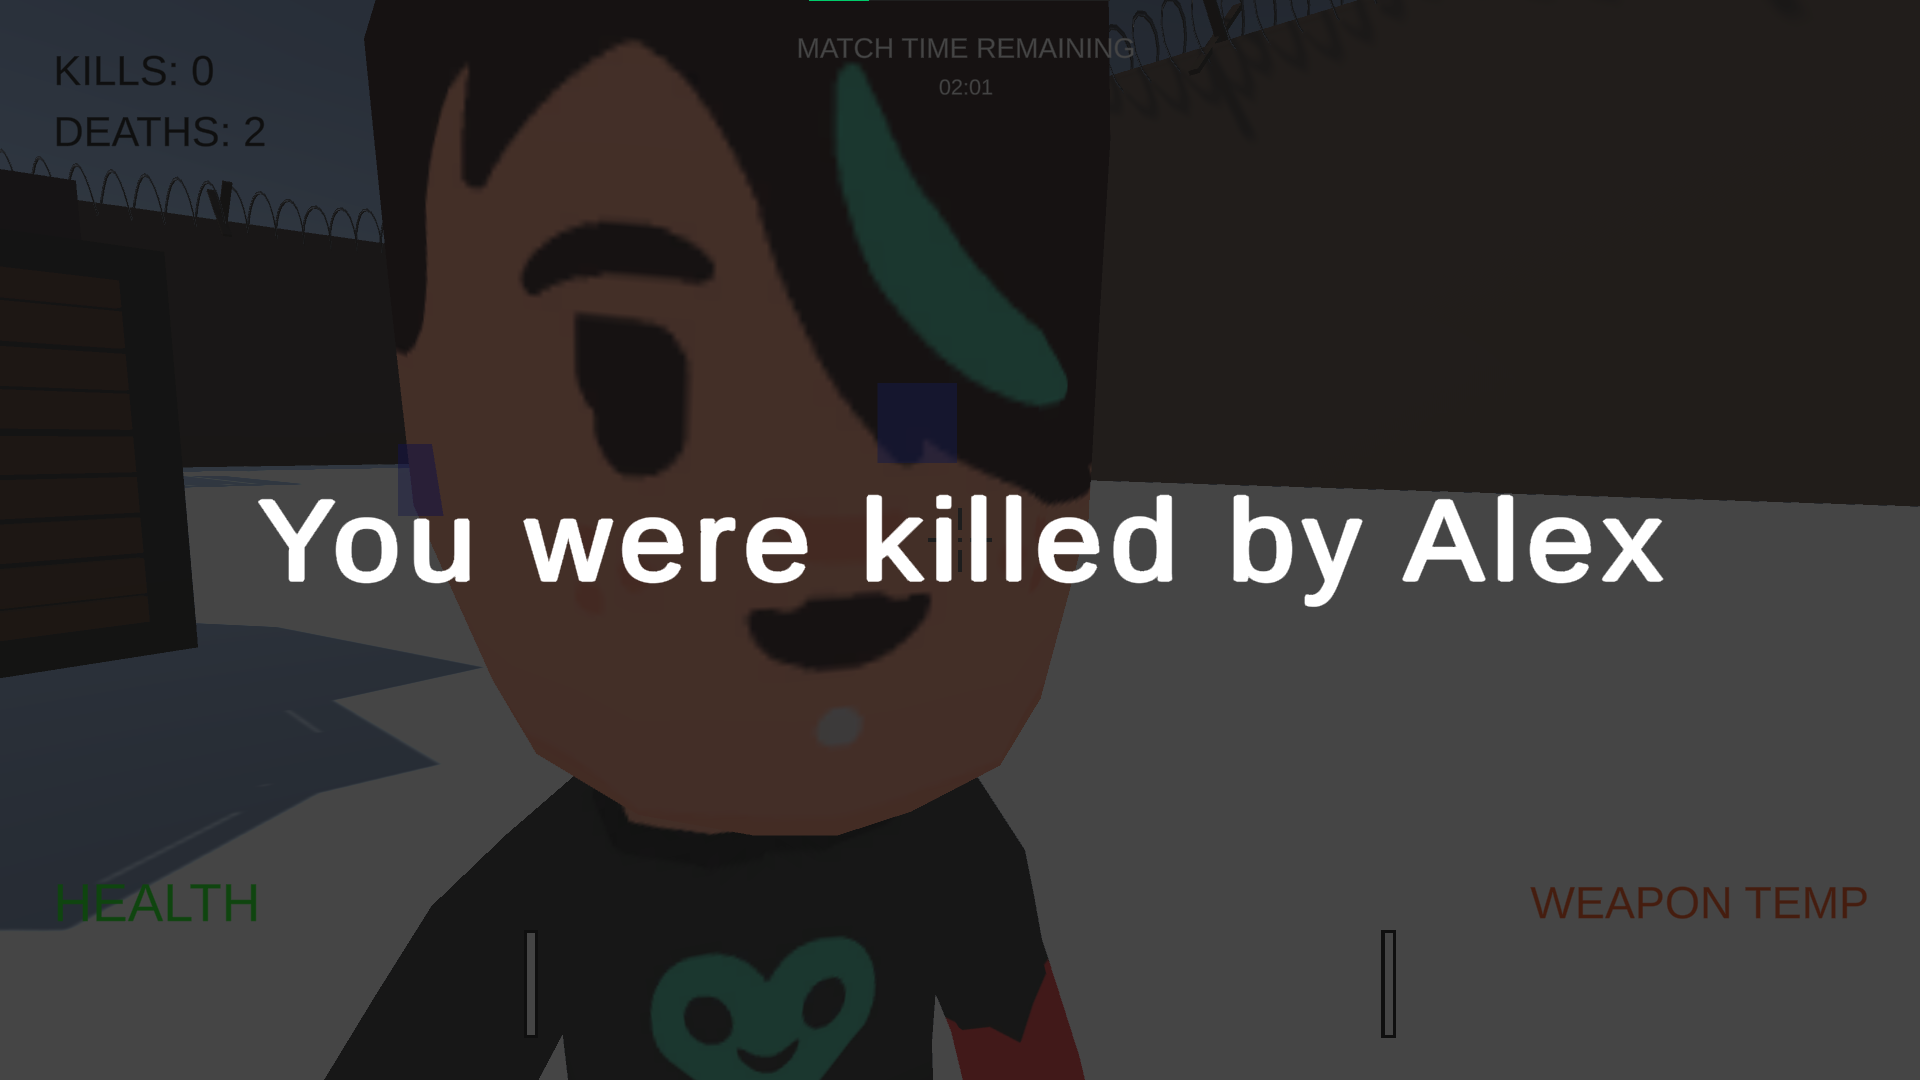
\includegraphics[width=10cm]{saatdibunuh.png}
        \caption{Tampilan Dibunuh}
        \label{fig:dibunuh}
    \end{figure}
\end{enumerate}
\newpage
\section{Pengujian Sistem}
\noindent

Pengujian sistem dilakukan untuk mengetahui fungsional menu utama sistem dari game jak meuprang dengan metode \textit{blackbox} testing.
\subsection{Pengujian Blackbox Testing}
\noindent

Pengujian blackbox untuk menguji fungsi sistem atau kekurangan pada 
perangkat lunak yang diuji agar menjadi lebih baik dan dapat diminimalisir 
terjadinya kekurangan pada sistem
\begin{enumerate}
    \item Tombol Cari Room \\
    % \usepackage{tabularray}
\begin{table}[h]
    \centering
    \caption{Hasil Pengujian Cari Room}
    \label{tb:tabel-cariroom}
    \begin{tblr}{
      vlines,
      hline{1,7} = {-}{0.08em},
      hline{2} = {-}{},
      hline{3-6} = {4,6}{},
    }
    ID  & {Rincian \\Pengujian} & {Hasil yang\\di harapkan}             & Player & {Hasil yang \\didapatkan}             & Keterangan \\
    R01 & {Tombol \\Cari Room}  & {Menampilkan \\Panel\\Pencarian Room} & 1      & {Menampilkan \\Panel\\Pencarian Room} & Berhasil   \\
        &                       &                                       & 2      &                                       & Berhasil   \\
        &                       &                                       & 3      &                                       & Berhasil   \\
        &                       &                                       & 4      &                                       & Berhasil   \\
        &                       &                                       & 5      &                                       & Berhasil   
    \end{tblr}
    \end{table}
    \newpage
    \item Tombol Buat Room \\
    \begin{table}[h]
        \centering
        \caption{Hasil Pengujian Buat Room}
        \label{tb:tabel-buatroom}
        \begin{tblr}{
          vlines,
          hline{1,7} = {-}{0.08em},
          hline{2} = {-}{},
          hline{3-6} = {4,6}{},
        }
        ID  & {Rincian \\Pengujian} & {Hasil yang\\di harapkan}                & Player & {Hasil yang \\didapatkan}               & Keterangan \\
        B01 & {Tombol\\Buat Room}   & {Menampilkan \\Panel Inputan\\Nama Room} & 1      & {Menampilkan\\Panel Inputan\\Nama Room} & Berhasil   \\
            &                       &                                          & 2      &                                         & Berhasil   \\
            &                       &                                          & 3      &                                         & Berhasil   \\
            &                       &                                          & 4      &                                         & Berhasil   \\
            &                       &                                          & 5      &                                         & Berhasil   
        \end{tblr}
        \end{table}
        \newpage
        \item Tombol Exit Room \\
        \begin{table}[h]
            \centering
            \caption{Hasil Pengujian Exit Room}
        \label{tb:tabel-exitroom}
            \begin{tblr}{
              vlines,
              hline{1,7} = {-}{0.08em},
              hline{2} = {-}{},
              hline{3-6} = {4,6}{},
            }
            ID  & {Rincian \\Pengujian} & {Hasil yang\\di harapkan}  & Player & {Hasil yang \\didapatkan} & Keterangan \\
            E01 & {Tombol\\Exit Room}   & {Menampilkan~\\Menu Utama} & 1      & {Menampilkan\\Menu utama} & Berhasil   \\
                &                       &                            & 2      &                           & Berhasil   \\
                &                       &                            & 3      &                           & Berhasil   \\
                &                       &                            & 4      &                           & Berhasil   \\
                &                       &                            & 5      &                           & Berhasil   
            \end{tblr}
            \end{table}
        \item Tombol About Game \\
        \begin{table}[h]
            \centering
            \caption{Hasil Pengujian About Game}
            \label{tb:tabel-aboutgame}
            \begin{tblr}{
              vlines,
              hline{1,7} = {-}{0.08em},
              hline{2} = {-}{},
              hline{3-6} = {4,6}{},
            }
            ID  & {Rincian \\Pengujian} & {Hasil yang\\di harapkan} & Player & {Hasil yang \\didapatkan} & Keterangan \\
            A01 & {Tombol\\About\\Game} & {Menampilkan\\Informasi}  & 1      & {Menampilkan\\Informasi}  & Berhasil   \\
                &                       &                           & 2      &                           & Berhasil   \\
                &                       &                           & 3      &                           & Berhasil   \\
                &                       &                           & 4      &                           & Berhasil   \\
                &                       &                           & 5      &                           & Berhasil   
            \end{tblr}
            \end{table}
        \newpage
        \item Tombol Keluar \\
        \begin{table}[h]
            \centering
            \caption{Hasil Pengujian Keluar Game}
            \label{tb:tabel-keluargame}
            \begin{tblr}{
              vlines,
              hline{1,7} = {-}{0.08em},
              hline{2} = {-}{},
              hline{3-6} = {4,6}{},
            }
            ID  & {Rincian \\Pengujian} & {Hasil yang\\di harapkan} & Player & {Hasil yang \\didapatkan} & Keterangan \\
            K01 & {Tombol\\Keluar}      & {Mengeluarkan\\Permainan} & 1      & {Mengeluarkan\\Permainan} & Berhasil   \\
                &                       &                           & 2      &                           & Berhasil   \\
                &                       &                           & 3      &                           & Berhasil   \\
                &                       &                           & 4      &                           & Berhasil   \\
                &                       &                           & 5      &                           & Berhasil   
            \end{tblr}
            \end{table}
\end{enumerate}

Pada Tabel \ref{tb:tabel-blackbox} untuk menampilkan menghitung persentase kelayakan menu game dari 5 pengguna.
\begin{table}[h]
    \centering
    \caption{Hasil Pengujian Blac Box}
    \label{tb:tabel-blackbox}
    \begin{tabular}{|ll|l|l|l|} 
    \toprule
    \multicolumn{1}{|l|}{\begin{tabular}[c]{@{}l@{}}Test\\Case\\Id\end{tabular}} & Penggunaan Berhasil                      & \begin{tabular}[c]{@{}l@{}}Pengunaan\\Tidak\\Berhasil\end{tabular} & Presentase & Hasil                 \\ 
    \hline
    R01                                                                          & 5                                        & 0                                                                  & $5/5 \times 100\%$  & 100\%                      \\ 
    \hline
    B01                                                                          & 5                                        & 0                                                                  & $5/5 \times 100\%$  & 100\%                      \\ 
    \hline
    E01                                                                          & 5                                        & 0                                                                  & $5/5 \times 100\%$  & 100\%                      \\ 
    \hline
    A01                                                                          & 5                                        & 0                                                                  & $5/5 \times 100\%$  & 100\%                      \\ 
    \hline
    K01                                                                          & 5                                        & 0                                                                  & $5/5 \times 100\%$  & 100\%                      \\ 
    \hline
                                                                                 & \multicolumn{1}{l}{Rata Rata Presentase} & \multicolumn{1}{l}{}                                               &            & 100\%  \\
    \bottomrule
    \end{tabular}
    \end{table}

    Berdasarkan tabel atas dijelaskan pengujian kelayakan menu utama game menggunakan 
metode black box dengan 5 pengguna didapatkan hasil 100% dari pengguna 
berhasil dan pengguna tidak berhasil.
\newpage
\section{Pengukuran QOS \textit{(Quality Of Service)}}
\noindent

Pengukuran QOS dilakukan untuk mengetahui performa jaringan dari photon unity networking.

\subsection{Pengukuran Packet Loss}
\noindent

Packet loss merupakan banyaknya paket yang gagal 
mencapai tempat tujuan paket tersebut dikirim. Ketika packet 
loss besar maka dapat diketahui bahwa jaringan sedang sibuk 
atau terjadi overload. Berdasarkan teori dan hasil pengamatan 
disaat melakukan pengukuran ,maka hasil yang didapatkan 
bisa dilihat pada \ref{tb:tabel-packetloss}.

\begin{table}[h]
    \centering
    \caption{Hasil Pengukuran Packet loss}
    \label{tb:tabel-packetloss}
    \begin{tabular}{|c|c|c|c|c|} 
    \hline
    No & \begin{tabular}[c]{@{}c@{}}Hari\\Tanggal\end{tabular}        & Pengujian & Packet Loss & Tiphon        \\ 
    \hline
    1  & \begin{tabular}[c]{@{}c@{}}Rabu\\26 July\\2023\end{tabular}  & 1         & 0,1\%       & Sangat Bagus  \\ 
    \hline
    2  & \begin{tabular}[c]{@{}c@{}}Rabu\\26 July\\2023\end{tabular}  & 2         & 0\%         & Sangat Bagus  \\ 
    \hline
    3  & \begin{tabular}[c]{@{}c@{}}Rabu\\26 July \\2023\end{tabular} & 3         & 0,6\%       & Sangat Bagus  \\ 
    \hline
    4  & \begin{tabular}[c]{@{}c@{}}Rabu\\26~July\\2023\end{tabular}  & 4         & 0,2\%       & Sangat Bagus  \\ 
    \hline
    5  & \begin{tabular}[c]{@{}c@{}}Rabu\\26~July\\2023\end{tabular}  & 5         & 0\%         & Sangat Bagus  \\
    \hline
    \end{tabular}
    \end{table}
\newpage
Dari hasil pengukuran packet loss menurut standar TIPHON jika rata-rata packet loss 
0 maka masuk kedalam kategori “Sangat Bagus”.
\subsection{Pengukuran Delay}
\noindent

Delay merupakan lamanya waktu yang dibutuhkan oleh 
data atau informasi untuk sampai ke tempat tujuan data atau 
informasi tersebut dikirim. Delay pada suatu jaringan akan 
menentukan langkah apa yang akan kita ambil ketika kita 
memanajemen suatu jaringan. Berdasarkan teori dan hasil 
pengamatan disaat melakukan pengukuran ,maka hasil yang 
didapatkan bisa dilihat pada \ref{tb:tabel-delay}

\begin{table}[h]
    \centering
    \caption{Hasil Pengukuran Delay}
    \label{tb:tabel-delay}
    \begin{tabular}{|c|c|c|c|c|} 
    \hline
    No & \begin{tabular}[c]{@{}c@{}}Hari\\Tanggal\end{tabular}        & Pengujian & \begin{tabular}[c]{@{}c@{}}Delay\\Average\end{tabular} & Tiphon        \\ 
    \hline
    1  & \begin{tabular}[c]{@{}c@{}}Rabu\\26 July\\2023\end{tabular}  & 1         & 125                                                    & Sangat Bagus  \\ 
    \hline
    2  & \begin{tabular}[c]{@{}c@{}}Rabu\\26 July\\2023\end{tabular}  & 2         & 110                                                    & Sangat Bagus  \\ 
    \hline
    3  & \begin{tabular}[c]{@{}c@{}}Rabu\\26 July \\2023\end{tabular} & 3         & 125                                                    & Sangat Bagus  \\ 
    \hline
    4  & \begin{tabular}[c]{@{}c@{}}Rabu\\26~July\\2023\end{tabular}  & 4         & 90                                                     & Sangat Bagus  \\ 
    \hline
    5  & \begin{tabular}[c]{@{}c@{}}Rabu\\26~July\\2023\end{tabular}  & 5         & 130                                                    & Sangat Bagus  \\
    \hline
    \end{tabular}
    \end{table}

    Dari hasil pengukuran delay untuk masing-masing 
pengguna adalah tertinggi terdapat di 1,3 dan 5 pengguna menurut standar TIPHON jika 
rata-rata delay dibawah 150 ms maka masuk kedalam kategori 
“Sangat Bagus”.
